\documentclass[,man,floatsintext]{apa6}
\usepackage{lmodern}
\usepackage{amssymb,amsmath}
\usepackage{ifxetex,ifluatex}
\usepackage{fixltx2e} % provides \textsubscript
\ifnum 0\ifxetex 1\fi\ifluatex 1\fi=0 % if pdftex
  \usepackage[T1]{fontenc}
  \usepackage[utf8]{inputenc}
\else % if luatex or xelatex
  \ifxetex
    \usepackage{mathspec}
  \else
    \usepackage{fontspec}
  \fi
  \defaultfontfeatures{Ligatures=TeX,Scale=MatchLowercase}
\fi
% use upquote if available, for straight quotes in verbatim environments
\IfFileExists{upquote.sty}{\usepackage{upquote}}{}
% use microtype if available
\IfFileExists{microtype.sty}{%
\usepackage{microtype}
\UseMicrotypeSet[protrusion]{basicmath} % disable protrusion for tt fonts
}{}
\usepackage{hyperref}
\hypersetup{unicode=true,
            pdftitle={Measuring Adults' and Children's Comprehension of Disjunction},
            pdfauthor={Masoud Jasbi~\& Michael C. Frank},
            pdfkeywords={conjunction, disjunction, implicatures, semantics, pragmatics, logical connectives, language, acquisition, development, children},
            pdfborder={0 0 0},
            breaklinks=true}
\urlstyle{same}  % don't use monospace font for urls
\usepackage{longtable,booktabs}
\usepackage{graphicx,grffile}
\makeatletter
\def\maxwidth{\ifdim\Gin@nat@width>\linewidth\linewidth\else\Gin@nat@width\fi}
\def\maxheight{\ifdim\Gin@nat@height>\textheight\textheight\else\Gin@nat@height\fi}
\makeatother
% Scale images if necessary, so that they will not overflow the page
% margins by default, and it is still possible to overwrite the defaults
% using explicit options in \includegraphics[width, height, ...]{}
\setkeys{Gin}{width=\maxwidth,height=\maxheight,keepaspectratio}
\IfFileExists{parskip.sty}{%
\usepackage{parskip}
}{% else
\setlength{\parindent}{0pt}
\setlength{\parskip}{6pt plus 2pt minus 1pt}
}
\setlength{\emergencystretch}{3em}  % prevent overfull lines
\providecommand{\tightlist}{%
  \setlength{\itemsep}{0pt}\setlength{\parskip}{0pt}}
\setcounter{secnumdepth}{0}
% Redefines (sub)paragraphs to behave more like sections
\ifx\paragraph\undefined\else
\let\oldparagraph\paragraph
\renewcommand{\paragraph}[1]{\oldparagraph{#1}\mbox{}}
\fi
\ifx\subparagraph\undefined\else
\let\oldsubparagraph\subparagraph
\renewcommand{\subparagraph}[1]{\oldsubparagraph{#1}\mbox{}}
\fi

%%% Use protect on footnotes to avoid problems with footnotes in titles
\let\rmarkdownfootnote\footnote%
\def\footnote{\protect\rmarkdownfootnote}


  \title{Measuring Adults' and Children's Comprehension of Disjunction}
    \author{Masoud Jasbi\textsuperscript{1}~\& Michael C. Frank\textsuperscript{2}}
    \date{}
  
\shorttitle{Measuring the Comprehension of Disjunction}
\affiliation{
\vspace{0.5cm}
\textsuperscript{1} Harvard University\\\textsuperscript{2} Stanford University}
\keywords{conjunction, disjunction, implicatures, semantics, pragmatics, logical connectives, language, acquisition, development, children\newline\indent Word count: X}
\usepackage{csquotes}
\usepackage{upgreek}
\captionsetup{font=singlespacing,justification=justified}

\usepackage{longtable}
\usepackage{lscape}
\usepackage{multirow}
\usepackage{tabularx}
\usepackage[flushleft]{threeparttable}
\usepackage{threeparttablex}

\newenvironment{lltable}{\begin{landscape}\begin{center}\begin{ThreePartTable}}{\end{ThreePartTable}\end{center}\end{landscape}}

\makeatletter
\newcommand\LastLTentrywidth{1em}
\newlength\longtablewidth
\setlength{\longtablewidth}{1in}
\newcommand{\getlongtablewidth}{\begingroup \ifcsname LT@\roman{LT@tables}\endcsname \global\longtablewidth=0pt \renewcommand{\LT@entry}[2]{\global\advance\longtablewidth by ##2\relax\gdef\LastLTentrywidth{##2}}\@nameuse{LT@\roman{LT@tables}} \fi \endgroup}


\usepackage{lineno}

\linenumbers
\usepackage{xcolor}

\authornote{All the experimental materials, data, randomization code, and analysis code for the studies reported in this paper are available in the following online repository: \url{https://github.com/jasbi/disjunction_comprehension}. The repository also includes instructions for reproducing this research.

Correspondence concerning this article should be addressed to Masoud Jasbi, Boylston Hall, Cambridge, MA. E-mail: \href{mailto:masoud_jasbi@fas.harvard.edu}{\nolinkurl{masoud\_jasbi@fas.harvard.edu}}}

\abstract{
Disjunction has had a key role in advancing theories of logic, language, and cognition. Previous research suggested that adults and preschool children might differ in their interpretation of linguistic disjunction in two ways. First, unlike adults, children might interpret a disjunction as conjunction. For example, children might consider a sentence like ``\emph{there is a cat or a dog}'' only true if there is both a cat and a dog. Second, children might interpret \emph{or} as inclusive disjunction when adults interpret it as exclusive. For example, adults may judge ``\emph{there is a cat or a dog}'' as false when both animals are present, but children consider it true. We first review the long tradition of research on children's development of disjunction. Then we present three studies that assess adults' and children's understanding of \emph{and} and \emph{or} in the same task, using three different measures: forced-choice binary truth value judgments, forced-chocie ternary truth value judgments, and free-form verbal feedback. \ldots{} The results suggest that forced-choice truth-value judgments may underestimate children's pragmatic competence. In order to capture children's semantic as well as pragmatic competence, we recommend complementing forced choice truth value judgment task with measures more sensitive to pragmatic infelicities.


}

\begin{document}
\maketitle

\hypertarget{introduction}{%
\section{Introduction}\label{introduction}}

When introducing disjunction to students of logic, Alfred Tarski (1941) complained about the complex factors that affect its comprehension in everyday language:

\begin{quote}
\enquote{The usage of the word \emph{or} in everyday English is influenced by certain factors of a psychological character. Usually we affirm a disjunction of two sentences only if we believe that one of them is true but wonder which one. If, for example, we look upon a lawn in normal light, it will not enter our mind to say that the lawn is green or blue, since we are able to affirm something simpler, and at the same time, stronger, namely that the lawn is green. Sometimes even, we take the utterance of a disjunction as an admission by the speaker that he does not know which of the members of the disjunction is true. (Tarski, 1941, p. 21)}
\end{quote}

In addition to this \textsc{ignorance} implication -- that the truth of neither disjunct is known -- Tarski (1941) noted that a disjunction has at least two different interpretations: exclusive and inclusive. Suppose, \enquote{a child has asked to be taken on a hike in the morning and to a theater in the afternoon, and we reply: No, we shall go on a hike or we shall go to the theater} (Tarski, 1941, p. 20). Tarski explained that disjunction in this example is \textsc{exclusive} because \enquote{we intend to comply with only one of the two requests} and not both. However, a disjunction may also have an \textsc{inclusive} interpretation like the following example: \enquote{Customers who are teachers or college students are entitled to a special reduction}. Tarski explained that \emph{or} in this example is inclusive \enquote{since it is not intended to refuse reduction to a teacher who is at the same time a college student.}

Grice (1975) provided an pragmatic explanation for the complex set of interpretations that linguistic disjunction receives. He argued that the literal meaning of \emph{or} (i.e.~its semantics) is captured by the truth conditions of logical inclusive disjunction. However, this literal meaning is enriched as speakers use a disjunction in context. Ignorance and exclusivity implications are inferences derived from our pragmatic reasoning on why the speaker used a disjunction. Grice (1975) generalized and systematized Tarski's intuition that we do not say \enquote{the lawn is green or blue} because we can say \enquote{something simpler and at the same time stronger}; namely \enquote{the lawn is green}. He suggested a general communicative principle: speakers strive to be as truthful, informative, relevant, and brief as they can. Therefore, a disjunctive assertion commonly results in the inference that the speaker could not have uttered only one of the disjuncts, because s/he was uncertain about its truth (ignorance inference). Similarly, exclusivity of a disjunction is inferred by reasoning about the speaker's choice of the connective (\emph{or} instead of \emph{and}). Going back to Tarski's example, the child can reason that her dad could have said \enquote{we are going on a hike \emph{and} we are going to the theater} if he intended to do both. He used \emph{or} instead. Assuming he knew whether he wants to do both or not, his utterance must mean he wants to do one or the other (exclusivity inference). Within the Gricean framework, ignorance and exclusivity of \emph{or} are secondary inferences, derived from the interaction of its literal (inclusive) meaning with conversational principles.

Complexities involved in the interpretation of disjunction have consequences for developmental theories. How does this intricate knowledge develop in humans? When do children begin to interpret a disjunction? What are their early interpretations like? Do they differ significantly from adult interpretations? Previous studies have suggested that preschool children (age 3-5 years) may differ in their interpretations of disjunction in two ways. First, they are more likely to interpret a disjunction word such as \emph{or} as a conjunction (Braine \& Rumain, 1981; Neimark, 1970; Singh, Wexler, Astle-Rahim, Kamawar, \& Fox, 2016; Tieu et al., 2016). Second, children are more likely to interpret a disjunction as inclusive. In other words, unlike adults, children do not compute exclusivity inferences, and therefore consider a disjunction as completely felicitous when both disjuncts are true (Chierchia, Crain, Guasti, Gualmini, \& Meroni, 2001; Chierchia et al., 2004; Crain, 2008).

In the present study, we tested adults' and children's comprehension of disjunction using two- and three-alternative forced-choice judgment tasks. We also collected children's spontaneous verbal responses in the same tasks. The results of our experiments suggested that children (and adults) differentiated linguistic disjunction and conjunction: overall, they did not interpret \emph{or} the way they interpreted \emph{and}. In the context of predicting an outcome, both adults and children considered a true disjunction to be of \enquote{intermediate felicity}: not wrong, but not completely right either. In adults, the infelicity of disjunction was better reflected in the judgment task with three alternatives, than the one with only two. In children, this infelicity was better reflected in their spontaneous verbal corrections, than their forced-choice judgments with either two or three alternatives. These results suggest that previously observed differences between adults and children's comprehension of disjunction may be at least partly due to the type of measurements used.

In the next section, we provide a broad review of the literature on children's acquisition of disjunction. We show that previous studies provide considerable support for the role of task design and measurement in shaping our conclusions regarding the development of disjunction. Experiment 1 tested adults in two- and three-alternative forced-choice tasks. Experiment 2 tested preschool children with a three-alternative forced choice judgment task. It also reports their spontaneous verbal feedback and corrections in the same task. Experiment 3 tested children's comprehension of disjuntion in a two-alternative forced-choice task and reported their spontaneous feedback and corrections as well. In General Discussion, we report our conclusions regarding these experiments and their consequences for theories of semantic and pragmatic development.

\hypertarget{litreview}{%
\subsection{Previous Research}\label{litreview}}

Children's comprehension of logical connectives \emph{and} and \emph{or} have been studied within two research programs. The first program, starting in 1960s, was inspired by Piaget's developmental theory (Inhelder \& Piaget, 1958) and focused on the emergence of logical concepts in humans. The second research program started in late 1990s and was inspired by Grice's theory of meaning. Rather than conceptual development, it focused on linguistic development, separating the roles of semantics and pragmatics in language acquisition. In this section, we briefly outline some of the main findings in these two research programs, summarizing how task design and measurement affected their conclusions.

Within the Piagetian program, researchers hypothesized that the abstract and logical notion of disjunction (i.e.~inclusive disjunction) is constructed from the more concrete concept of \enquote{choice between two options}. The prediction was that until the age of 11 (concrete operational stage), children understand a disjunction like \enquote{A or B} as \enquote{one of the two options}. This is similar to an exclusive meaning for disjunction. After age 11 (formal operational stage), children start to form abstract logical concepts and interpret \enquote{A or B} as inclusive. To examine this hypothesis, researchers conducted large scale in-class tests of school children and college students (Neimark \& Slotnick, 1970; Nitta \& Nagano, 1966). Participants were presented with pictures of objects and asked to circle those described by a statement such as \enquote{not bird}, \enquote{bird and white}, \enquote{bird or white}. These studies concluded that the majority of the participants understood negation and conjunction, but only college students correctly answered statements with disjunction. They reported that participants made two types of \enquote{errors}. First across all ages, some participants interpreted disjunction as conjunction. Second, some participants interpreted disjunction as exclusive. Based on these results Neimark (1970) concluded that a \enquote{correct} (inclusive) understanding of disjunction only develops in the high school years and depends on the attainment of formal operations as defined in the Piagetian theory\footnote{The term \enquote{error} has different definitions in the literature on the comprehension of disjunction. Early studies considered any response other than an inclusive interpretation as erroneous. More importantly, what counted as an error was decided by researchers. Today, however, both exclusive and inclusive interpretations are considered correct and the conjunctive interpretation is more likely to be considered erroneous. Researchers also focus more on adult-like vs.~non-adult-like behavior in children rather than \enquote{errorneous} behavior. Depending on the context, a disjunction may be interpreted as exclusive, inclusive, or even conjunctive, and adults set the benchmark interpretation for children's performance in experimental tasks.}.

Further investigations suggested that the conjunctive errors may be due to the task design of in-class tests. Paris (1973) reported that in his in-class truth-judgment task, even a fifth of college students did not differentiate \emph{or} from \emph{and}, interpreting both as conjunction. He attributed these conjunctive interpretations of \emph{or} to the application of non-linguistic strategies when the task is difficult or confusing (See Clark, 1973 for a discussion of nonlinguistic strategies in child language acquisition). He explained that children in his task (as well as some adults) were probably \enquote{comparing visual and auditory information with little regard for the implied logical relationship in the verbal description.} In a disjunction such as \enquote{A or B}, participants responded with \enquote{true} if the individual disjuncts (A, B) matched the pictures and false otherwise. Such a non-linguistic matching strategy would yield correct answers for conjunction but incorrect (conjunctive) answers for disjunction. This account also explains why in Paris (1973)'s study, conjunctive readings reduced with age and why using the word \emph{either} along with \emph{or} helped reduce conjunctive interpretations further.

Further evidence for the task-dependent nature of conjunctive readings or \enquote{errors} come from \enquote{give-item} tasks. Suppes and Feldman (1969) provided children with wooden blocks of different colors and shapes and used commands such as \enquote{give the things that are round or green.} They found that depending on the exact phrasing of the command, preschool children can interpret a disjunction as exclusive or conjunctive. However, using a similar \enquote{give-item} task, Johansson and Sjolin (1975)'s did not find considerable conjunctive interpretations. They tested Swedish-speaking children's comprehension of disjunction in present tense sentences such as \enquote{Richard wants to drink lemonade or milk. Show me what he drank!} and imperative sentences such as \enquote{Put up {[}the picture of{]} the car or the doll!}. They reported that children, as young as four years of age, interpreted a disjunction as exclusive. Based on these findings, Johansson and Sjolin (1975) argued that the linguistic \emph{or} should be kept separate from the logical notion of (inclusive) disjunction. While linguistic understanding of \emph{or} develops early as exclusive disjunction, the logical understanding of it (as inclusive disjunction) develops late.

Braine and Rumain (1981) tested participants with both a simplified replication of Suppes and Feldman (1969)'s \enquote{give-item} task and a version of what is today known as the truth value judgment task. For their replication of Suppes and Feldman (1969), they reported that both children and adults provided a \enquote{choose-one} (i.e.~exclusive) interpretation of disjunction. They did not find any conjunctive interpretations, providing even further support for the role of task design. However, this was not the case in the truth value judgment task. In this task, a puppet described the contents of four boxes, each containing four animal toys. For example, the puppet said \enquote{Either there is a horse or a duck in the box.} The first box had both animals, the second had only a horse, the third only a duck, and the last had neither. Participants were asked if the puppet was right. The results showed that adults were split between an inclusive and an exclusive interpretation of disjunction. The 7 to 10 year-olds were more likely to consider the disjunction as inclusive. However, the youngest group (5-6 years old) was most likely to interpret a disjunction similar to a conjunction: they said the puppet was right when both animals were in the box and not right or partly right if only one of the animals was in the box. Following Paris (1973), Braine and Rumain (1981) argued that in this task, younger children do not take the contribution of the connective \emph{or} into account. Instead, they use a non-linguistic strategy in which the disjunction is right if both propositions are true, partly right if only one is true, and wrong if neither is true. Braine and Rumain (1981) concluded that children's ability to interpret a disjunction in a command develops earlier than their ability to judge its truth values.

In Braine and Rumain (1981)'s judgment task, the puppet uttered a disjunction even though the content of the box was known to both the puppet and the participant (i.e.~speaker lacked ignorance). As Tarski (1941) noted, such uses of disjunction sound odd and infelicitous. This may have contributed to the application of a non-linguistic strategy and resulted in conjunctive readings. Later truth value judgment studies such as Chierchia, Crain, Guasti, and Thornton (1998) controlled for this effect of disjunction by making the puppet utter disjunction as a prediction of an unknown event, and let participants judge the prediction after they see the outcome. Furthermore, Chierchia et al. (1998) argued that in order to truly capture children's semantic competence with \emph{or}, experiments need to test its comprehension in contexts that do not invite exclusivity implicatures. These contexts include embedding \emph{or} under linguistic operators such as negation or conditionals.

Since Chierchia et al. (1998)'s arguments, numerous studies within the Gricean program have tested preschool children's comprehension of disjunction in embedded contexts as varied as negative sentences (Crain, Gualmini, \& Meroni, 2000), conditional sentences (Gualmini, Crain, \& Meroni, 2000), restriction and nuclear scope of the universal quantifier \emph{every} (Chierchia et al., 2001, 2004), nuclear scope of the negative quantifier \emph{none} (Gualmini \& Crain, 2002), restriction and nuclear scope of \emph{not every} (Notley et al., 2012a), and prepositional phrases headed by \emph{before} (Notley et al., 2012b), as well as similar environments in other languages such as Mandarin Chinese and Japanese (Goro \& Akiba, 2004; Su, 2014; Su \& Crain, 2013). These studies almost unanimously support the hypothesis that the inclusive interpretation emerges earlier than the exclusive interpretation. This conclusion stands in sharp contrast to the earlier conclusions from the give-item tasks, however. Since under the Gricean account, the exclusive interpretation of disjunction is the result of pragmatic (scalar) implicatures, the earlier emergence of inclusive interpretations is considered consistent with evidence from development of quantifier implicatures. (Barner, Brooks, \& Bale, 2011; Noveck, 2001; Papafragou \& Musolino, 2003).

Methodological issues qualify this seemingly strong conclusion, however. As mentioned earlier, Braine and Rumain (1981) found that the same children were more likely to interpret a disjunction as exclusive in a give-item task and inclusive/conjunctive in a truth value judgment task. Therefore, truth value judgment tasks may not reveal the full picture regarding children' knowledge of exclusivity implicatures. Furthermore, several studies listed above test children's knowledge of disjunction in environments that largely collapse the distinction between \emph{and} and \emph{or}. For example, in the restriction of \emph{every}, a conjunction and a disjunction can result in the same interpretation (e.g. \emph{Every man or woman is happy} vs. \emph{Every man and woman is happy}). \textcolor{red}{Therefore, successful interpretation in such studies can also be achieved by a nonlinguistic strategy such as ignoring the contribution of *or* and independently checking the truth of  each proposition, as discussed by earlier studies} (Braine \& Rumain, 1981; Paris, 1973).

\textcolor{red}{More recently, two truth value judgment studies reported that the majority of preschool children in their sample interpreted a disjunction similar to a conjunction} (Singh et al., 2016, and @tieu2016). To control for ignorance, Tieu et al. (2016) used the \enquote{prediction mode} of the Truth Value Judgment Task, in which the puppet provides a prediction or guess. Then an event occurs and participants are asked if the prediction was right. For example, there was a chicken on the screen and two toy objects, for example a bus and a plane. The puppet appeared on the screen and predicted that \enquote{the chicken pushed the bus or the plane}. Then the chicken pushed either one or both of the objects. Participants stamped on a happy face or a sad face to show whether the puppet's guess was right or wrong. They reported that unlike adults, preschool children were more likely to consider a disjunction as \enquote{right} when both disjuncts were true, rather than only one. They concluded that children - the majority of them in their sample - interpreted disjunction as conjunction. They hypothesized that this conjunctive interpretaton of disjunction is due to children's non-adult-like pragmatic enrichments.

However, a recent replication of Tieu et al. (2016) by Skordos, Feiman, Bale, and Barner (n.d.) suggests that the high rate of conjunctive interpretations were most likely due to the experimental context's lack of plausible dissent: the experiment did not provide conditions under which utterances could be deemed false plausibly. They tested preschoolers in two conditions: replication (two-alternatives) and three-alternatives. The first condition was a direct replication of Tieu et al. (2016). The three-alternatives condition provided three objects; for example a plane, a bus, and a bicycle. The reasoning was that if there are only two objects, a disjunction is trivially true, and consequently children may consider that unacceptable. The results replicated Tieu et al. (2016)'s findings in the replication condition, but showed that conjunctive interpretations of disjunction disappeared almost completely in the three-alternatives condition. Skordos et al. (n.d.) concluded that children's conjunctive interpretations are most likely due to non-linguistic strategies applied when they are uncertain about some aspect of the experimental task. This conclusion is similar to the conclusions of Paris (1973) and Braine and Rumain (1981) in early studies of disjunction.

\begin{longtable}[]{@{}ll@{}}
\caption{\label{tab:conclusionsReview} Summary of tasks used in previous studies and their conclusions}\tabularnewline
\toprule
\begin{minipage}[b]{0.42\columnwidth}\raggedright
Task\strut
\end{minipage} & \begin{minipage}[b]{0.52\columnwidth}\raggedright
Conclusion\strut
\end{minipage}\tabularnewline
\midrule
\endfirsthead
\toprule
\begin{minipage}[b]{0.42\columnwidth}\raggedright
Task\strut
\end{minipage} & \begin{minipage}[b]{0.52\columnwidth}\raggedright
Conclusion\strut
\end{minipage}\tabularnewline
\midrule
\endhead
\begin{minipage}[t]{0.42\columnwidth}\raggedright
\textbf{School test (Imperative)} \newline \textit{Circle all that are bird or black!}\strut
\end{minipage} & \begin{minipage}[t]{0.52\columnwidth}\raggedright
Comprehension of \emph{or} develops in high school. Before that children often interpret it as conjunction.\strut
\end{minipage}\tabularnewline
\begin{minipage}[t]{0.42\columnwidth}\raggedright
\textbf{School test (Truth Value Judgment)} \newline \textit{The bird is in the nest or the shoe is on the foot.}\strut
\end{minipage} & \begin{minipage}[t]{0.52\columnwidth}\raggedright
Children (8-14 years) as well as some adults interpret \emph{or} as a conjunction. This is likely due to task demands and application of nonlinguistic strategies.\strut
\end{minipage}\tabularnewline
\begin{minipage}[t]{0.42\columnwidth}\raggedright
\textbf{Give-item} \newline \textit{Give me all the green things or give me all the round things.}\strut
\end{minipage} & \begin{minipage}[t]{0.52\columnwidth}\raggedright
Children (4-7 years) interpret disjunction as exclusive (choose-one). The inclusive (logical) concept of disjunction develops later.\strut
\end{minipage}\tabularnewline
\begin{minipage}[t]{0.42\columnwidth}\raggedright
\textbf{Give-item + Truth Value Judgment} \newline \textit{Give me all the green things or give me all the round things.} \newline \textit{Either there is X or there is Y in the box.}\strut
\end{minipage} & \begin{minipage}[t]{0.52\columnwidth}\raggedright
Children (5-6 years) interpret \emph{or} as exclusive in commands but ignore its contribution in truth value judgments and interpret it as a conjunction. Interpretation of disjunction in commands develops earlier than the knowledge of its truth conditions.\strut
\end{minipage}\tabularnewline
\begin{minipage}[t]{0.42\columnwidth}\raggedright
\textbf{Truth Value Judgment (controling for Speaker Ignorance)} \newline \textit{A troll ate a piece of pizza or an ice cream.}\strut
\end{minipage} & \begin{minipage}[t]{0.52\columnwidth}\raggedright
Children (4-6 years) understand \emph{or} as inclusive disjunction. Two studies report majority conjunctive interpretations too.\strut
\end{minipage}\tabularnewline
\begin{minipage}[t]{0.42\columnwidth}\raggedright
\textbf{Truth Value Judgment (controling for Speaker ignorance and Number of alternatives)}\strut
\end{minipage} & \begin{minipage}[t]{0.52\columnwidth}\raggedright
Children (4-6 years) understand the truth conditions of \emph{or} similar to inclusive disjunction. No evidence for conjunctive interpreations.\strut
\end{minipage}\tabularnewline
\bottomrule
\end{longtable}

To summarize, our review of previous literature suggests that the design of an experimental task can have a big impact on our conclusions about children's comprehension of disjunction (Table \ref{tab:conclusionsReview}). First, different tasks may be more or less suitable for capturing different interpreations of disjunction. For example, the \enquote{Give-item} task can successfully capture exclusive interpretations, while the TVJT task is more successful in capturing inclusive interpretations. Second, regardless of task type, increased task demands or infelicitous use of disjunction can result in increased conjunctive interpretations of disjunction. With the give-item task, Suppes and Feldman (1969) found a considerable rate of conjunctive interpretations, but these interpretations disappeared in Braine and Rumain (1981)'s more simplified replication. Similarly, Tieu et al. (2016) reported that a large number of children interpreted \emph{or} as \emph{and}, but these conjunctive readings also disapppeared when Skordos et al. (n.d.)'s replication controlled for the number of alternatives in the task. Therefore, previous studies highlight the role of task design and measurement in studying children's comprehension of disjunction. More specifically and with respect to conjunctive interpretations of disjunction, previous studies provide substantial evidence linking them to task design. Therofere, while it is plausible to consider non-adult-like pragmatic computations as a cause of conjunctive readings of disjunctio in children, it is important to first conclusively rule out the influence of task design.

\hypertarget{present-study}{%
\subsection{Present Study}\label{present-study}}

The goal of this study was to further simplify task design and measure children's comprehension of disjunction in multiple ways. We used simple existential sentences (e.g. \emph{there is a cat or a dog}) and tested the interpretation of participants in a card game. The game controlled for the role of speaker ignorance, by making the speaker guess what was on a card without seeing it. It used trials with the conjunction word \emph{and}, as well as adult participants as controls. Children's interpretations were measured in three different ways: a two-alternative forced choice task (2AFC), a three-alternative forced choice task, and the analysis of children's free-form verbal responses in each task. Table \ref{tab:study1info} provides the summary of methods used in Experiments 1, 2, and 3.

\begin{longtable}[]{@{}lllll@{}}
\caption{\label{tab:study1info}Summary of Expeirment 1, 2 and 3 methods}\tabularnewline
\toprule
\begin{minipage}[b]{0.16\columnwidth}\raggedright
Study\strut
\end{minipage} & \begin{minipage}[b]{0.01\columnwidth}\raggedright
N\strut
\end{minipage} & \begin{minipage}[b]{0.17\columnwidth}\raggedright
Age\strut
\end{minipage} & \begin{minipage}[b]{0.17\columnwidth}\raggedright
Mode\strut
\end{minipage} & \begin{minipage}[b]{0.34\columnwidth}\raggedright
Response Options\strut
\end{minipage}\tabularnewline
\midrule
\endfirsthead
\toprule
\begin{minipage}[b]{0.16\columnwidth}\raggedright
Study\strut
\end{minipage} & \begin{minipage}[b]{0.01\columnwidth}\raggedright
N\strut
\end{minipage} & \begin{minipage}[b]{0.17\columnwidth}\raggedright
Age\strut
\end{minipage} & \begin{minipage}[b]{0.17\columnwidth}\raggedright
Mode\strut
\end{minipage} & \begin{minipage}[b]{0.34\columnwidth}\raggedright
Response Options\strut
\end{minipage}\tabularnewline
\midrule
\endhead
\begin{minipage}[t]{0.16\columnwidth}\raggedright
Experiment 1\strut
\end{minipage} & \begin{minipage}[t]{0.01\columnwidth}\raggedright
57\strut
\end{minipage} & \begin{minipage}[t]{0.17\columnwidth}\raggedright
Adults\strut
\end{minipage} & \begin{minipage}[t]{0.17\columnwidth}\raggedright
Online (Mturk)\strut
\end{minipage} & \begin{minipage}[t]{0.34\columnwidth}\raggedright
Wrong, Right\strut
\end{minipage}\tabularnewline
\begin{minipage}[t]{0.16\columnwidth}\raggedright
\strut
\end{minipage} & \begin{minipage}[t]{0.01\columnwidth}\raggedright
52\strut
\end{minipage} & \begin{minipage}[t]{0.17\columnwidth}\raggedright
Adults\strut
\end{minipage} & \begin{minipage}[t]{0.17\columnwidth}\raggedright
Online (Mturk)\strut
\end{minipage} & \begin{minipage}[t]{0.34\columnwidth}\raggedright
Wrong, Kinda Right, Right\strut
\end{minipage}\tabularnewline
\begin{minipage}[t]{0.16\columnwidth}\raggedright
Experiment 2\strut
\end{minipage} & \begin{minipage}[t]{0.01\columnwidth}\raggedright
42\strut
\end{minipage} & \begin{minipage}[t]{0.17\columnwidth}\raggedright
3;1-5;2, M=4;3\strut
\end{minipage} & \begin{minipage}[t]{0.17\columnwidth}\raggedright
Study Room\strut
\end{minipage} & \begin{minipage}[t]{0.34\columnwidth}\raggedright
Circle (Wrong), Little Star (Little Right), Big Star (Right)\strut
\end{minipage}\tabularnewline
\begin{minipage}[t]{0.16\columnwidth}\raggedright
Experiment 3\strut
\end{minipage} & \begin{minipage}[t]{0.01\columnwidth}\raggedright
50\strut
\end{minipage} & \begin{minipage}[t]{0.17\columnwidth}\raggedright
3;6-5;9, M=4;7\strut
\end{minipage} & \begin{minipage}[t]{0.17\columnwidth}\raggedright
Study Room\strut
\end{minipage} & \begin{minipage}[t]{0.34\columnwidth}\raggedright
Yes (Right), No (Wrong) + Open-ended Feedback\strut
\end{minipage}\tabularnewline
\bottomrule
\end{longtable}

\hypertarget{study1}{%
\section{Experiment 1: Adult's 2AFC and 3AFC Judgments}\label{study1}}

This study examines adults' comprehension of \emph{or}, and uses it as a benchmark for children's comprehension in Experiments 2 and 3. We tested adults in both two-alternative and three-alternative forced choice tasks (2AFC and 3AFC).

\hypertarget{methods}{%
\subsection{Methods}\label{methods}}

\hypertarget{participants}{%
\subsubsection{Participants}\label{participants}}

109 English speaking adults participated via Amazon Mechanical Turk (MTurk). 57 of them were assigned to a 2AFC judgment task and 52 to a 3AFC judgment task. In the 2AFC task, participants had to judge using the options \enquote{wrong} and \enquote{right}. In the 3AFC task they had to choose between \enquote{wrong}, \enquote{kinda right}, and \enquote{right}\footnote{There are many possible labels for the middle option on a scale, including \enquote{kinda right}, \enquote{kinda wrong}, or \enquote{neither}. A later experiment, tested different intermediate labels and found that adults consider \enquote{kinda right} to be a more suitable option for capturing pragmatic infelicities (see Jasbi, Waldon, \& Degen, 2019). We expect similar behavior from labels that refer to non-maximal degrees of being \enquote{right} such as \enquote{a bit right} or \enquote{a little right}.}. The two conditions were otherwise identical. The task took about 5 minutes on average to complete. At the end of the study, participants received \$0.4 as compensation.

\hypertarget{stimuli}{%
\subsubsection{Stimuli}\label{stimuli}}

We used six cards, each with one or two cartoon animals on them. Three cards had one animal and three cards had two (Figure \ref{fig:stimuli} in Appendix). We represent these six cards with animal names in small caps: \textsc{cat, dog, ele, cat+dog, cat+ele, dog+ele} (\textsc{ele} stands for elephant). In each trial, a card was shown to the participant and a blindfolded cartoon character guessed what animal was on the card. The guess was either a simple existential sentence (e.g. \emph{There is a cat}), one with a conjunction (e.g. \emph{There is a cat and a dog}), or one with a disjunction (e.g. \emph{There is a cat or a dog}). In this paper we use the short forms \enquote{\emph{cat}}, \enquote{\emph{cat and dog}}, and \enquote{\emph{cat or dog}} to represent these guesses. Crossing the different types of cards and guesses results in 12 different possible trial types. We chose 8 trial types, balancing the number of one-animal vs.~two-animal cards, simple vs.~connective guesses, and (expected) true vs.~false trials.

Figure \ref{fig:trialtypes} shows our trial types using example cards as rows and example utterances as columns. Control trials consisted of simple guesses (e.g. \emph{elephant}, \emph{cat}) with cards that had one animal (e.g. \textsc{cat}) or two animals (e.g. \textsc{cat+dog}). In half of these trials the description was true and in half it was false. When two animals are on the card (e.g. \textsc{cat+dog}) and one is guessed (e.g. \emph{cat}), the guess could be false if interpreted exhaustively (e.g. \textbf{only} \emph{cat}). In addition to acting as a control, such trials could show how often children make exhaustive inferences. Conjunction trials (e.g. \emph{cat and dog}) were controls for disjunction trials. Half of conjunction trials were false and half true (false when only one animal was on the card and true when both were.) Finally, disjunction trials constituted the critical trials of our experiments. When two animals were on the card (e.g. \textsc{cat+dog}), a disjunction guess (e.g. \emph{cat or dog}) could be true if interpreted inclusively (e.g. \emph{cat or dog, or both}), and false if interpreted exclusively (e.g. \emph{cat or dog}, \textbf{not both}).

\begin{figure}

{\centering 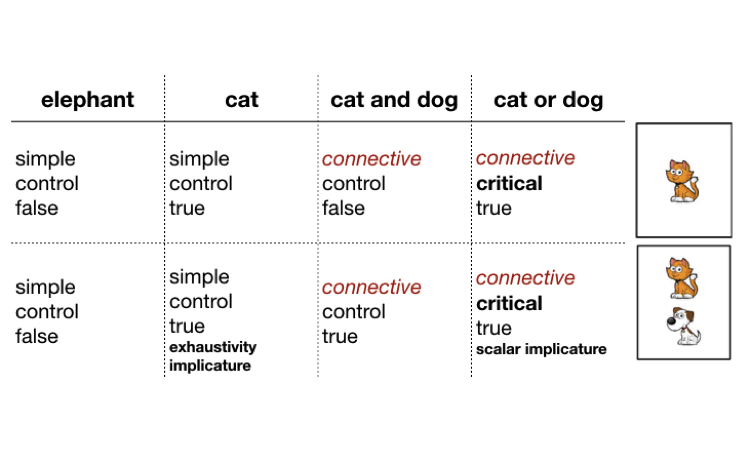
\includegraphics{Jasbi-Frank-2019_files/figure-latex/trialtypes-1} 

}

\caption{Control and critical trial types in the connective guessing game. Rows show example cards and columns example utterances (guesses).}\label{fig:trialtypes}
\end{figure}

\hypertarget{procedure}{%
\subsubsection{Procedure}\label{procedure}}

The experiment had three phases: introduction, instruction, and test. In the introduction, participants saw the six cards and read that they would play a guessing game. Then a blindfolded cartoon character named Bob appeared on the screen. Participants were told that in each round of the game, they would see a card and Bob was going to guess what animal was on the card. The study emphasized that Bob could not see anything. Participants were asked to judge whether Bob's guess was right. In the instruction phase, participants saw an example trial where a card with the image of a dog was shown with the following sentence written above Bob's head: \emph{There is a cat on the card}. All participants correctly responded with \enquote{wrong} and proceeded to the test phase. In the test phase, participants saw one trial per trial type. Within each trial type, the specific card and guess were chosen at random. The order of trial types was also randomized. Figure \ref{fig:stimuli} in the appendix shows an example test trial.

\hypertarget{results}{%
\subsection{Results}\label{results}}

\begin{figure}
\centering
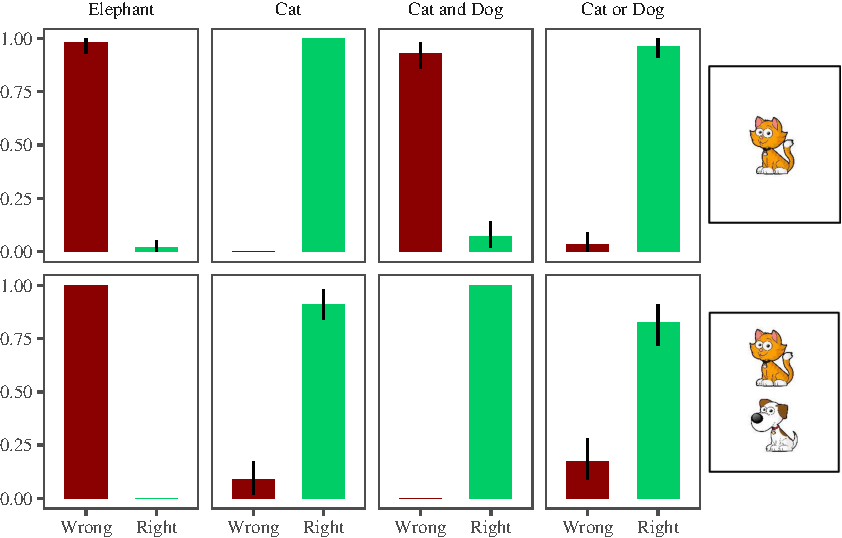
\includegraphics{Jasbi-Frank-2019_files/figure-latex/binaryAdultsPlot-1.pdf}
\caption{\label{fig:binaryAdultsPlot}Adults' two-alternative forced choice judgments in Experiment 1.}
\end{figure}

Figure \ref{fig:binaryAdultsPlot} shows the results for the adult 2AFC task. The two left columns show the simple guesses and serve as controls. The results show that if the guessed animal (e.g. \emph{elephant}) was not on the card (e.g. \textsc{cat/cat+dog}), participants judged the guess as \enquote{wrong}. If the guessed animal was on the card (e.g. \emph{cat}), participants judged the guess to be \enquote{right}. The next two columns of Figure \ref{fig:binaryAdultsPlot} show the results for the test conditions, namely conjunction and disjunction. A conjunction (e.g. \emph{cat and dog}) was considered \enquote{wrong} if only one of the animals was on the card (e.g. \textsc{cat}), and \enquote{right} if both were (e.g. \textsc{cat+dog}). A disjunction (e.g. \emph{cat or dog}) was \enquote{right} whether one or both animals were on the card (e.g. \textsc{cat/cat+dog}). The patterns of \enquote{right} and \enquote{wrong} responses in the two-alternative task match the expectations for truth and falsehood of conjunction and inclusive disjunction.

\begin{figure}
\centering
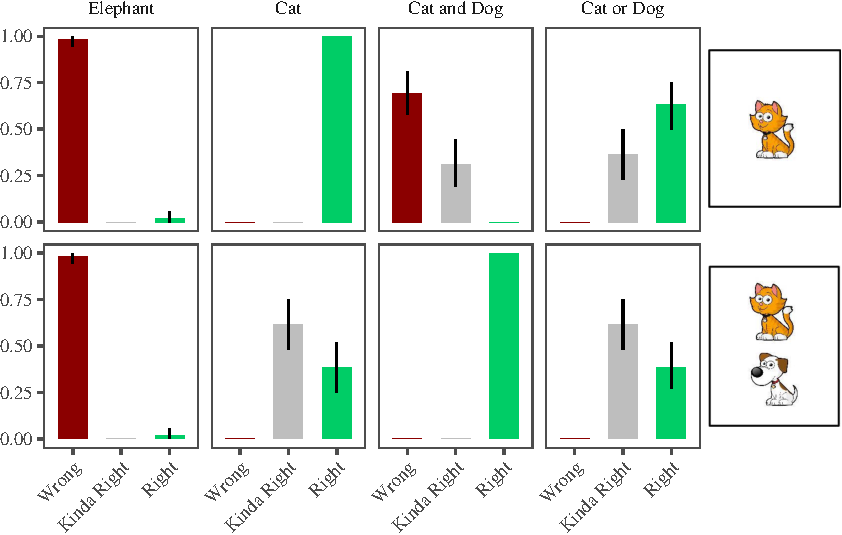
\includegraphics{Jasbi-Frank-2019_files/figure-latex/ternaryAdultsPlot-1.pdf}
\caption{\label{fig:ternaryAdultsPlot}Adults' three-alternative forced choice judgments in Experiment 1.}
\end{figure}

Figure \ref{fig:ternaryAdultsPlot} shows the results for the 3AFC judgment task. The addition of an intermediate response option affected the results in some trial types but not others. If the animal mentioned (e.g. \emph{elephant}) was not on the card (e.g. \textsc{cat/cat+dog}), participants judged the guess as \enquote{wrong}, regardless of the number of response options. Similarly, if the animal(s) mentioned (e.g. \emph{cat}, \emph{cat and dog}) perfectly matched the one(s) on the card (e.g. \textsc{cat}, \textsc{cat+dog}), participants judged the guess as \enquote{right} in both 2AFC and 3AFC tasks. Judgments for such trial types had an extreme nature (completely wrong/right) and not an intermediate one.

The four remaining trial types showed different patterns of judgments in the 2AFC and the 3AFC tasks. If one animal was mentioned (e.g. \emph{cat}) but two animals were on the card (e.g. \textsc{cat+dog}), participant judgments were divided between \enquote{right} and \enquote{kinda right}. When only one animal was on the card (e.g. \textsc{cat}) and the guess was a conjunction (e.g \emph{cat and dog}), most adults considered the guess \enquote{wrong} but some chose \enquote{kinda right}, possibly suggesting that the intermediate option was used to express partial truth of a guess. With disjunction guesses (e.g. \emph{cat or dog}), responses were split between \enquote{kinda right} and \enquote{right}.

It is likely that for the different disjunction trial-types, participants had different reasons to consider them not completely right. When only one animal was on the card (e.g.~cat), particiopants may have considered a simple guess (e.g. \emph{there is a cat}) as completely right. When two animals were on the card (e.g.~cat and dog), participants may have expected the connective \emph{and} instead of \emph{or}. As we shall see in the next two experiments, children explicitly mention these alternatives in their open-ended (free-form) responses.

\hypertarget{discussion}{%
\subsection{Discussion}\label{discussion}}

\begin{longtable}[]{@{}lllll@{}}
\caption{\label{tab:truthtable} Truth conditions of conjunction, inclusive, disjunction, and exclusive disjunction. \enquote{cat} and \enquote{dog} represent the propositions that \enquote{there is a cat} and \enquote{there is a dog} on the card respectively.}\tabularnewline
\toprule
cat & dog & cat \(\land\) dog & cat \(\lor\) dog & cat \(\oplus\) dog\tabularnewline
\midrule
\endfirsthead
\toprule
cat & dog & cat \(\land\) dog & cat \(\lor\) dog & cat \(\oplus\) dog\tabularnewline
\midrule
\endhead
T & T & T & T & F\tabularnewline
T & F & F & T & T\tabularnewline
F & T & F & T & T\tabularnewline
F & F & F & F & F\tabularnewline
\bottomrule
\end{longtable}

Consider the truth conditions for conjunction and disjunction shown in Table \ref{tab:truthtable}. A conjunction is true when both conjuncts are true and false otherwise. An inclusive disjunction is true when at least one disjunct is true, and false otherwise. An exclusive disjunction is true when only one of the disjuncts is true and false otherwise. Let's also assume a simple linking function in which false statements are judged as \enquote{wrong} and true statements as \enquote{right} (see Jasbi et al. (2019) for a discussion of linking assumptions in such a task). In Experiment 1, this purely truth-conditional account has the following predictions: First, conjunction guesses like \enquote{cat and dog} are wrong when only one of the animals is on the card and right when both are. Second, disjunction guesses are always right if they are interpreted as inclusive (because in all disjunction trials at least one of the animals was on the card). However, if disjunction is interpreted as exclusive, it should be judged as wrong when both animals are on the card. Finally, if truth conditions are all that matters, the addition of the intermediate option \enquote{kinda right} should not substantially affect the judgments.

The results of the 2AFC and 3AFC tasks in Experiment 1 support two conclusions. First, judgments for \emph{and} matched logical conjunction and \emph{or} inclusive disjunction. If adults in our task interpreted \emph{or} as strictly exclusive, we expected majority \enquote{wrong} responses when both disjuncts were true. Yet neither task showed substantial \enquote{wrong} responses for disjunction trials. Second, addition of an intermediate option affected response patterns in some trial-types. These trials fell into two major categories. First, those with responses split between \enquote{wrong} and \enquote{kinda right}. Second, those with responses split between \enquote{kinda right} and \enquote{right}. The first category of responses, namely the split between \enquote{wrong} and \enquote{kinda right}, only happened when there was one animal on the card (e.g. \textsc{cat}) and the guess was a conjunction (e.g. \emph{cat and dog}). In such trials, even though the guess was false, it was not completely incorrect; one of the animals was guessed right. Therefore, choosing the intermediate option could reflect the judgment that such guesses are better than those that fail to name any animal on the card.

The second category corresponds to trial types in which the guesses were literally true, but underinformative. When there were two animals on the card (e.g. \textsc{cat+dog}), guessing only one of them (e.g. \emph{cat}) or guessing a disjunction of them (e.g. \emph{cat or dog}) results in a true yet sub-optimal statement. In these cases, there was a better possible guess, namely a conjunction (e.g. \emph{cat and dog}). Similarly, when only one animal was on the card (e.g. \textsc{cat}), and Bob guessed a disjunction (e.g. \emph{cat or dog}), the guess was true but not the best one. A simple utterance (e.g. \emph{there is a cat}) would have been better. Therefore, disjunction guesses (with either one or both disjuncts being true) had intermediate acceptability. This is generally the case in the context of guessing and prediction: a guess or prediction with a disjunction may be true but it is not the most informative guess. There is always a better or more specific guess.

In a forced choice task with no intermediate option, participants may differ on how they respond to cases of intermediate acceptaiblity. Some may decide to ignore the slight unacceptability and focus on the truth of the statement. Others may decide to focus on the fact that a better guess was not made and express this in their judgments. This decision is independent of a participant's judgment of the linguistic stimuli, and depends on several factors including what matters for the purpuses of the task and what type of measurment is used. For example, in a two-alternative task, most adults may not consider non-truth-conditional violations grave enough to render a guess as \enquote{wrong}. Therefore, judgments in a 2AFC task match the truth of a guess. However, if a third intermediate option is provided, participants may opt to also express the unacceptaiblity or infelicity of a guess in the task - depending on the label of the intermediate option. In a subsequent study, we found that participants opt for the intermediate option more often if it is labeled as \enquote{kinda right} rather than \enquote{neither} (Jasbi et al., 2019). Most importantly, children may differ from adults in how they approach intermediate judgments in forced choice tasks. This source of variation between children and adults has remained relatively unexplored, despite previous evidence for it (Katsos, 2014; Katsos \& Bishop, 2011). The next two experiments provide evidence that children may differ from adults in how they deal with the intermediate nature of disjunction in forced-choice tasks.

\hypertarget{study2}{%
\section{Experiment 2: Children's three-alternative forced choice judgments vs.~open-ended verbal feedback}\label{study2}}

This experiment tested children's comprehension of disjunction in the same guessing game and compared them to those of adults'. Since the 3AFC judgment task in Experiment 1 was better at capturing the nuances of adults' pragmatic reasoning, we decided to first test children with the 3AFC task. We also provide an analysis of children's open-ended and sponteaneous verbal feedback to the guesses.

\hypertarget{methods-1}{%
\subsection{Methods}\label{methods-1}}

\hypertarget{participants-1}{%
\subsubsection{Participants}\label{participants-1}}

We recruited 42 English speaking children from the Bing Nursery School at Stanford University. Children were between 3;1 and 5;2 years old (Mean = 4;3).

\hypertarget{materials}{%
\subsubsection{Materials}\label{materials}}

We used the same set of cards and linguistic stimuli as the ones in study 1. There were 8 trial types and 2 trials per trial type for a total of 16 trials. We made two changes to make the experiment more suitable for children. First, instead of the fictional character Bob, a puppet named Jazzy played the guessing game with them. Jazzy wore a sleeping mask over his eyes during the game (Figure \ref{fig:jazzy}). Second, a pilot study showed that a scale with three alternatives is better understood and used by children if it is presented in the form of rewards to the puppet rather than verbal responses such as \enquote{wrong}, \enquote{a little bit right}, and \enquote{right}, or even hand gestures such as thumbs up, middle, and down. Therefore, we placed a set of red circles, small blue stars, and big blue stars in front of the children. These tokens were used to reward the puppet after each guess. During the introduction, the experimenter explained that if the puppet was right, the child should give him a big star; if the puppet was a little bit right, a little star, and if he was not right, a red circle. Katsos and Bishop (2011) \textcolor{red} {was the first study to use three types of rewards as response options (small strawberry, big strawberry, huge strawberry) to test preschool children's semantic and pragmatic competence. They reported that children used the intermediate response option when an utterance was pragmatically infelicitous.}

\hypertarget{procedure-1}{%
\subsubsection{Procedure}\label{procedure-1}}

The experiment was carried out in a quiet room with a small table and two small chairs. Children sat on one side of the table and the experimenter and the puppet on the other side facing the children. The groups of circles, small stars, and big stars were placed in front of the child from left to right respectively. A deck of six cards was in front of the experimenter. Similar to study 1 with adults, study 2 had three phases: introduction, instruction, and test.

The goal of the introduction was for the experimenter to show the cards to the children and make sure they recognized the animals and knew their names. The experimenter showed the cards to the children and asked them to label each animal. All children recognized the animals and could label them correctly. In the instruction phase, children went through three example trials. The experimenter explained that he was going to play with the puppet first, so that the child could learn the game. He removed the six introduction cards and placed a deck of three cards face-down on the table. From top to bottom (first to last), the cards had the following images: \textsc{cat}, \textsc{ele}, \textsc{cat+dog} (Table \ref{tab:instruction}). The experimenter put the sleeping mask on the puppet's eyes and explained that the puppet is going to guess what animal is on the cards. He then picked the first card and asked the puppet: \enquote{What do you think is on this card?} The puppet replied with \enquote{\emph{There is a dog}}. The experimenter showed the \textsc{cat}-card to the child and explained that when the puppet is \enquote{not right} he gets a circle\footnote{The pilot study had shown that some children struggle with understanding the word \enquote{wrong}, so \enquote{not right} was used instead.}. He then asked the child to give the puppet a circle. Rewards were collected by the experimenter and placed under the table to not distract the child. The second trial followed the same pattern except that the puppet guessed \enquote{right} and the experimenter invited the child to give the puppet a big star. In the final trial of the instruction, the puppet guessed that \emph{there is a cat} on the card when the card was \textsc{cat+dog}. The experimenter said that the puppet was \enquote{a little right} and asked the child to give him a little star.

In the test phase, the experimenter removed the three instruction cards and placed a deck of 16 randomized cards on the table. He explained that it was the child's turn to play with the puppet. For each card, the puppet provided a guess and the child provided the puppet with a reward. The guesses were paired with each card in a way that allowed two trials per 8 trial types\footnote{A more detailed description of the procedure as well as the randomization code for the test phase is available on the study's online repository.}.

\hypertarget{feedbackCoding}{%
\subsubsection{Offline Annotations}\label{feedbackCoding}}

While playing the game, children often provided spontaneous verbal reactions to the puppet's guesses. During the analysis of the videos, these verbal responses were categorized into four types: 1. None, 2. Judgments, 3. Descriptions, and 4. Corrections. The first category referred to cases where children did not say anything and only rewarded the puppet. The second cateogry (judgments) referred to positive/negative linguistic feedback that did not include information about the animals on the card. Examples include: \enquote{you are right!}, \enquote{yes}, \enquote{nope}, or \enquote{you winned!}. In the third category (descriptions), children labeled the animals on the card: \enquote{cat!}, \enquote{dog and elephant!}, \enquote{There is a cat and a dog!} etc. Finally, with correction, children provided extra \enquote{focus words} such as \emph{just}, \emph{only}, and emphasized \emph{AND} that acted like corrections to what the puppet had said. Examples include: \enquote{Just a cat!}, \enquote{Both!}, \enquote{The two are!}, \enquote{Only cat!}, \enquote{cat AND dog} (with emphasis placed on \emph{and}). In trials where the child provided both judgments as well as descriptions or corrections (e.g. \enquote{Yes! Cat!}), we placed the feedback into the more informative categories, namely description or correction.

\hypertarget{results-1}{%
\subsection{Results}\label{results-1}}

\hypertarget{truth-value-judgments}{%
\subsubsection{Truth Value Judgments}\label{truth-value-judgments}}

\begin{figure}
\centering
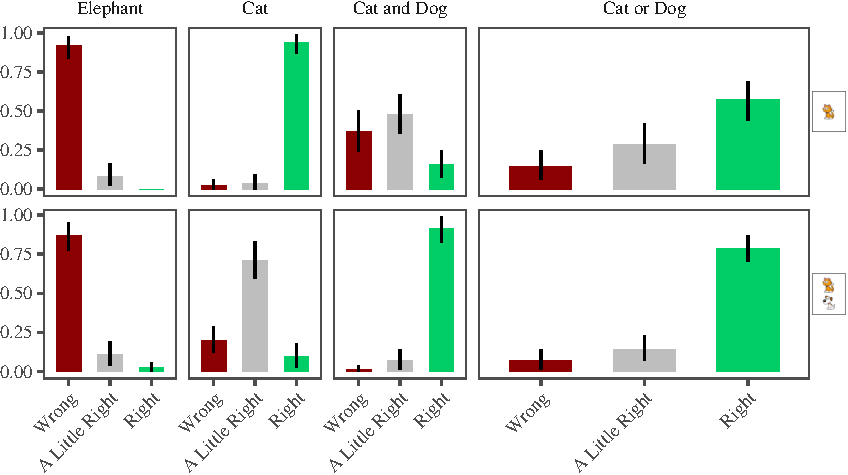
\includegraphics{Jasbi-Frank-2019_files/figure-latex/childrenTernaryPlot-1.pdf}
\caption{\label{fig:childrenTernaryPlot}Children's three-alternative forced-choice judgments in Experiment 2.}
\end{figure}

Figure \ref{fig:childrenTernaryPlot} shows the results for children's 3AFC judgments. Starting with control trials (leftmost column in Figure \ref{fig:childrenTernaryPlot}), if the mentioned animal (e.g. \emph{elephant}) was not on the card, children judged the guess as \enquote{wrong}. If the mentioned animal (e.g. \emph{cat}) was the only animal on the card, children judged the guess to be \enquote{right}. Here we ignore the results for exhaustivity trial types in which the animal mentioned (e.g. \emph{cat}) was only one of the animals on the card (e.g. \textsc{cat+dog}). The reason is that such trials were used in the instruction phase to introduce the \enquote{little bit right} option, and the results are probably biased by the instructions. With conjunction guesses (e.g. \emph{cat and dog}), when only one of the animals was on the card (e.g. \textsc{cat}), most children judged the guess as \enquote{wrong} or \enquote{a little right}. However, if both animals were on the card (e.g. \textsc{cat+dog}), they judged the conjunction as \enquote{right}. With disjunction guesses (e.g. \emph{cat or dog}), when only one of the animals mentioned was on the card (e.g. \textsc{cat}), children considered the guess \enquote{right} or \enquote{kinda right}. If both animals were on the card (e.g. \textsc{cat+dog}), the disjunction was considered \enquote{right}.

\begin{figure}
\centering
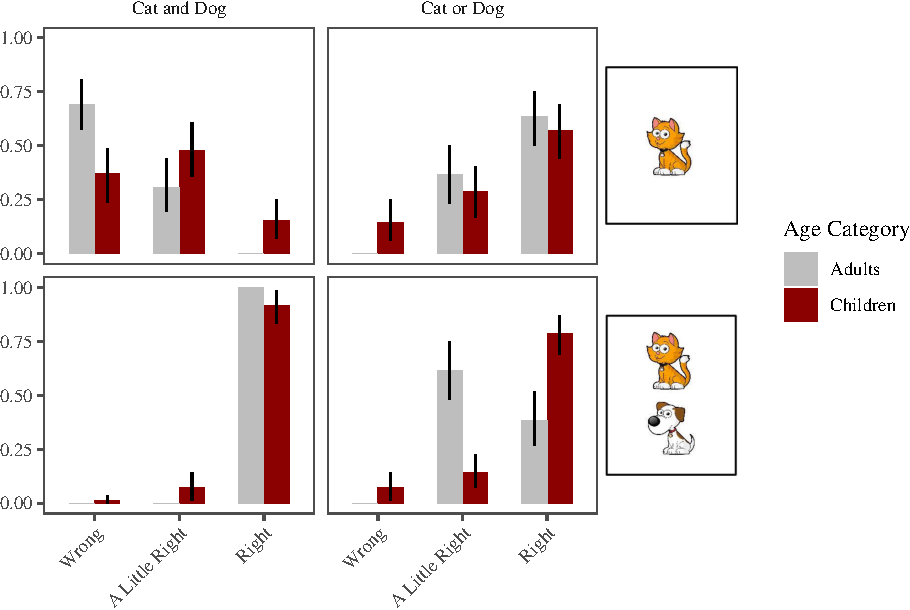
\includegraphics{Jasbi-Frank-2019_files/figure-latex/childAdultComp-1.pdf}
\caption{\label{fig:childAdultComp}Comparison of Adults' 3AFC judgments from Experiment 1 and Children's 3AFC judgments from Experiment 2.}
\end{figure}

MIKE--\textgreater{}

Figure \ref{fig:childAdultComp} compares the results for children and adults' 3AFC judgments in the conjunction and disjunction trials. Overall, the results look very similar. To quantify possible differences between adults and children more precisely and model both our 3AFC task as well as the subject-level clustering of data, we decided to fit ordinal mixed-effects logistic models. We adopted the Bayesian framework and used the R package \enquote{brms} (Bürkner, 2017).

First, we fit separate ordinal mixed-effects logistic models for adults and children. The models included the fixed effect of trial-type and maximal random-effects structures (Barr, Levy, Scheepers, \& Tily, 2013), i.e.~random intercepts and slopes for participants and items (cards).\footnote{response \textasciitilde{} trial type + (1 + trial type\textbar{}sid) + (1 + trial type\textbar{}card)} Second, we fit an ordinal mixed-effects model to the combined dataset of adults and children with the added interaction effect of \enquote{age category} (adult vs.~child), with \enquote{adults} set as the intercept.\footnote{response \textasciitilde{} trial type * age category + (1 + trial type\textbar{}sid) + (1 + trial type\textbar{}card)} For all models, the response variable had three ordered levels: \enquote{wrong}, \enquote{kinda right}, and \enquote{right}. The trial types \enquote{two animals, \emph{and}}, \enquote{two animals, \emph{or}}, and \enquote{one animal, \emph{and}} constituted the (dummy-coded) fixed effects of the model, with \enquote{one animal, \emph{or}} set as the intercept. The priors over trial types were set to \(\mathcal{N}(0,10)\). For other parameters, default weakly informative priors -- Student-t (3, 0, 10) and Cholesky LKJ Correlation (1) -- were used as endorsed in \enquote{brms} documantation. All four chains converged after 4000 samples (with a burn-in period of 2000 samples).

\begin{figure}
\centering
\includegraphics{Jasbi-Frank-2019_files/figure-latex/exp2TVJTstats-1.pdf}
\caption{\label{fig:exp2TVJTstats}Left: The mean and 90\% highest posterior density interval for the coefficients estimated in separate ordinal logistic regressions for adults and children, Right: Mean and 90\% highest posterior density interval for the interaction coefficients in the combined dataset.}
\end{figure}

The left panel of Figure \ref{fig:exp2TVJTstats} shows the mean and 90\% highest posterior density intervals (HPDIs) for three contrasts of interest estimated from separate ordinal models for adults and children. Because predictors were dummy-coded, it is possible to examine contrasts of interest by computing the difference between coefficients for pairs of conditions we wish to contrast. The x-axis shows the contrasts between the following trial-types: conjunction vs.~disjunction trials when only one animal was on the card (one animal, and-or), trials with one vs.~two animals on the card when the guess was a disjunction (or, two-one animal), and conjunction vs.~disjunction trials when two animals were on the card (two animals, and-or). Adults' and children's estimated coefficients are similar in sign to one another in the first and third contrasts, though adults' are more extreme. The first contrast (one animal, and-or) suggests that when only one animal was on the card, both adults and children had lower judgments for guesses with conjunction compared to guesses with disjunction. The third contrast suggests that when two animals were on the card, conjunction received higher judgments. For the second contrast, adults show negative values while children show positive values. This suggests that when the guess was a disjunction, children had slightly higher ratings when both animals were on the card compared to only one; adults on the other hand had slighly lower ratings and were more likely to choose \enquote{kinda right} over \enquote{right}. This is consistent with the hypothesis that children \enquote{compute exclusivity implicatures} at a lower rate than adults and are more likely to consider a disjunction acceptable when both disjuncts are true (Barner et al., 2011; Noveck, 2001; Papafragou \& Musolino, 2003). However, we will see that children's spontaneous feedback does not support this hypothesis.

To understand the extent to which children's judgments differed from adults' we will look at the mean and the 90\% HPDIs of the interaction coefficients from the combined model shown in the right panel of Figure \ref{fig:exp2TVJTstats}. We use this model to focus on the likely reliable differences between children and adults. Based on the 90\% HPDIs, we can infer that judgments of adults and children differed in two ways. First, when the guess was a disjunction (e.g. \emph{cat or dog}) and two animals were on the card (e.g. \textsc{cat+dog}), children gave higher ratings than adults. This is again related to the issue of exclusivity implicatures discussed before. Second, when the guess was a conjunction (e.g. \emph{cat and dog}) but only one animal was on the card (e.g. \textsc{cat}), children gave slightly higher ratings than adults did. This could be either due to children's judgments being more lenient or their judgments focusing more on matching lables to pictures rather than the connective. We will see more evidence for the label matching hypothesis in Experiment 3. \textless{}--MIKE

\hypertarget{spontaneous-open-ended-feedback}{%
\subsubsection{Spontaneous open-ended feedback}\label{spontaneous-open-ended-feedback}}

We also categorized and annotated children's spontaneous and free-form verbal reactions to the puppet's guesses. Table \ref{tab:feedbackCat} summarizes the definitions and examples for each category and Figure \ref{fig:exp2feedbackPlot} shows the results. We should point out that each trial type had a similar number of \enquote{None} cases. Some children remained silent throughout the experiment and only provided rewards to the puppet. In Experiment 3, we explicitly asked children to provide feedback and therefore, had no \enquote{None} response category. In the discussion and analysis here we will not comment further on the \enquote{None} category but focus on the other three categories.

\begin{figure}
\centering
\includegraphics{Jasbi-Frank-2019_files/figure-latex/exp2feedbackPlot-1.pdf}
\caption{\label{fig:exp2feedbackPlot}Children's open-ended Feedback in Experiment 2.}
\end{figure}

Starting with control trials (the leftmost column), when the guessed animal was not on the card (e.g. \emph{elephant}), children either provided judgments like \enquote{No!} or described what was on the care: \enquote{cat} or \enquote{cat and dog}. However, when the guessed animal (e.g. \emph{cat}) was the only animal on the card (e.g. \textsc{cat}), most children provided a positive judgment like \enquote{Yes}. When the animal guessed (e.g. \emph{cat}) was only one of the animals on the card (e.g. \textsc{cat+dog}), children described what was on the card, for example \enquote{cat and dog}.

In trials with conjunction (e.g. \emph{cat and dog}), children showed a high rate of corrections and descriptions when there was only one animal on the card (e.g. \textsc{cat}). In their corrections, children used the focus particles \emph{just} and \emph{only} as in \enquote{just a cat} or \enquote{only a cat}. When both animals were on the card (e.g. \textsc{cat+dog}) and a conjunction was used (e.g. \emph{cat and dog}), children predominantly provided positive judgments like \enquote{Yes!} and \enquote{You are right}. With disjunction (e.g. \emph{cat or dog}), when only one of the animals was on the card (e.g. \textsc{cat}), most children simply described what was on the card, saying for example \enquote{cat}. However, when both animals were on the card (e.g. \textsc{cat+dog}), children corrected the puppet by saying \enquote{Both!} or emphasizing \emph{and} as in \enquote{cat AND dog!}.

\begin{figure}
\centering
\includegraphics{Jasbi-Frank-2019_files/figure-latex/exp2FeedbackStats-1.pdf}
\caption{\label{fig:exp2FeedbackStats}The mean and 90\% highest posterior density interval of the coefficients of interest in experiment 2's mixed-effects multinomial logistic model on children's feedback.}
\end{figure}

MIKE----\textgreater{}To quantify and compare the distribution of children's feedback in different trial-types, we used a Bayesian mixed-effects multinomial regression model with the fixed effect of trial-type as well as random intercepts and slopes for participants and items (cards). The dependent measure was children's feedback categories of judgment, description, and correction, with correction set as the reference category. The trial types \enquote{one animal, \emph{or}}, \enquote{one animal, \emph{and}}, and \enquote{two animals, \emph{and}} constituted the (dummy-coded) fixed effects of the model with \enquote{two animals, \emph{or}} set as the intercept. Priors and convergence information were identical to those reported for our previous models.

Figure \ref{fig:exp2FeedbackStats} shows the mean and 90\% HPDIs of the multinomial model co-efficients, with the x-axis separating trial types. Starting from the left, the HPDIs for judgments and descriptions over corrections for the \enquote{one animal, and} trial-type included zero. This suggests that the feedback distribution was similar in conjunction trials with one animal and disjunction trials with two animals. Both trial types received a relatively high number of corrections. Considering the \enquote{one animal, \emph{or}} trials, the HPDIs for judgments and descriptions over corrections included zero but in the case of descriptions, only very marginally so. As we will see in the next experiment's replication of children's feedback, children provide more descriptions than corrections when only one of the disjuncts is true. Finally with \enquote{two animal, \emph{and}} trials, the HPDI for descriptions over corrections covers zero while that of judgments over corrections stays above zero. This suggests that when a conjunction was used and both animals were on the card, children provided more affirmative judgments than corrections. Overall, our statistical modeling suggests that patterns of children's feedback were similar for conjunction trials when only one proposition was true and disjunction trials when both propositions were true. In such trial-types children provided higher rates of corrections than other trial-types.\textless{}----MIKE

\hypertarget{discussion-1}{%
\subsection{Discussion}\label{discussion-1}}

In study 2, we used a 3AFC judgment task to test children's comprehension of logical connectives \emph{and} and \emph{or}. We compared these results to those found in the 3AFC judgment task of study 1 with adults. The general comparison showed that adults and children had similar patterns of judgments, except when both disjuncts were true. In such cases, adults judged the disjunctive guess as not completely right while most children judged it as completely right. There was even a slight preference among children to rewarded the puppet more in such cases, compared to cases of disjunction when only one disjunct was true.

To consider another measure of children's comprehension, we also looked at children's spontaneous open-ended verbal feedback to the puppet's guesses. Our analyses suggested that children recognized false and infelicitous utterances with the connectives and provided appropriate corrective feedback. As expected from an adult-like understanding of connectives, children corrected the puppet most often when there was only one animal on the card and the guess was conjunctive, or when there were two animals on the card and the guess was disjunctive. Perhaps the most important finding was that children increased their corrective feedback in disjunctive guesses where both disjuncts were true, compared to those with only one true disjunct. These findings differ from the results of the 3AFC judgment task, which suggested that children did not find any infelicity with disjunctive guesses when both disjuncts were true.

The analysis of children's open-ended feedback raises two important issues. First, it runs counter to what the 3AFC judgment task suggests with respect to exclusivity implicatures. The forced-choice task suggests that children find such underinformative utterances as unproblematic while analysis of their spontaneous feedback shows that they provided more corrections to such utterances. Second, one of the explanations for why children fail to derive implicatures is that they cannot access the stronger alternative to the disjunction word \emph{or}, namely \emph{and} (Barner et al., 2011). However, in the context of the guessing game, some children explicitly mentioned the word \emph{and}, as the word the puppet should have said instead of \emph{or}. Interestingly, these children continued to reward the puppet and considered the guess \enquote{right}, even though they corrected him. This raises the possibility that forced-choice truth value judgments underestimate children's pragmatic knowledge. In study 3, we used both a 2AFC truth judgment task and an analysis of children's open-ended feedback. If the findings of study 2 were on the right track, we expected to replicate the same pattern in study 3, and find that children's open-ended feedback better reflects their sensitivity to pragmatic violations than the results of the 2AFC judgments.

\hypertarget{study3}{%
\section{Experiment 3: Children's 2AFC judgments and open-ended feedback}\label{study3}}

This study used the same paradigm as Experiment 2 but measured children's judgments using a binary forced choice task. Similar to Experiment 2, children's open-ended feedback was also analyzed. The main hypothesis was that preschool children provide corrective feedback to the puppet if both disjuncts are true, but they do not consider this infelicity to be grave enough to render the guess \enquote{wrong} in a 2AFC judgment task. The main hypothesis along with relevant analyses and predictions were preregistered in an \enquote{As Predicted} format\footnote{The As Predicted PDF document is accessible at \url{https://aspredicted.org/x9ez2.pdf}.}.

\hypertarget{methods-2}{%
\subsection{Methods}\label{methods-2}}

\hypertarget{participants-2}{%
\subsubsection{Participants}\label{participants-2}}

We recruited 50 English speaking children from the Bing Nursery School at Stanford University. Children were between 3;6 and 5;9 years old (Mean = 4;7).

\hypertarget{materials-1}{%
\subsubsection{Materials}\label{materials-1}}

Experiment 3 was similar to Experiment 2 but differed in how children provided their judgments. Based on the findings in Experiment 2, we first focused on verbal feedback, instead of forced-choice responses. We used two different ways of measuring children's judgments. First, we encouraged children to provide verbal feedback to the puppet. They were asked to say \enquote{yes} when the puppet was right and \enquote{no} when he was not right. Importantly, they were also asked to help him say it better. In each trial, after children were done with this initial open-ended feedback, we asked the classic truth value judgment forced choice question: \enquote{Was Jazzy (the puppet) right?}. This question elicited a 2AFC response for each trial independent of children's earlier open-ended response. These two measures allowed us to compare open-ended and binary forced-choice judgments in the same paradigm and for the same trials.

\hypertarget{procedure-2}{%
\subsubsection{Procedure}\label{procedure-2}}

The setup and procedure were similar to Experiment 2, except there were no rewards. As in previous studies, participants sat through three phases: introduction, instruction, and test. The introduction phase made sure children knew the names of the animals on the cards. In the instruction phase, they received four training trials, as shown in Table \ref{tab:instructionStudy3} in the Appendix section.

As in Experiment 2, the experimenter put a sleeping mask over the puppet's eyes and explained that Jazzy (the puppet) was going to guess what animal was on the cards. He then picked the first card and asked the puppet: \enquote{What do you think is on this card?} The puppet replied with \enquote{There is a dog}. The experimenter showed the cat-card to the child and said: when Jazzy is \enquote{not right}, tell him \enquote{no}. He then asked the child to say \enquote{no} to the puppet. The second trial followed the same pattern except that the puppet guessed \enquote{right} and the experimenter invited the child to say \enquote{yes} to the puppet. There were two more instruction trials before the test phase began. The test phase contained 16 randomized trials, half of which contained guesses with the words \emph{and} and \emph{or}\footnote{The randomization code as well as the details of the methods are available on this paper's online repository.}.

\hypertarget{results-2}{%
\subsection{Results}\label{results-2}}

We first look at the results of the 2AFC judgement task for each trial type and compare them to those of the adults' in Experiment 1. Then we analyze children's open-ended responses and compare them to the forced choice responses obtained in the same trial types. For the 2AFC judgments we excluded 26 trials (out of total 800) where children either did not provide a Yes/No response or provided both (i.e. \enquote{Yes and No}). The exclusions were almost equally distributed among different types of guesses and cards. In the analysis of children's open-ended feedback, we excluded 8 trials (out of total 800) where children either did not provide any feedback or their feedback could not be categorized into the existing categories.

\hypertarget{two-alternative-forced-choice-judgments}{%
\subsubsection{Two-Alternative Forced Choice Judgments}\label{two-alternative-forced-choice-judgments}}

\begin{figure}
\centering
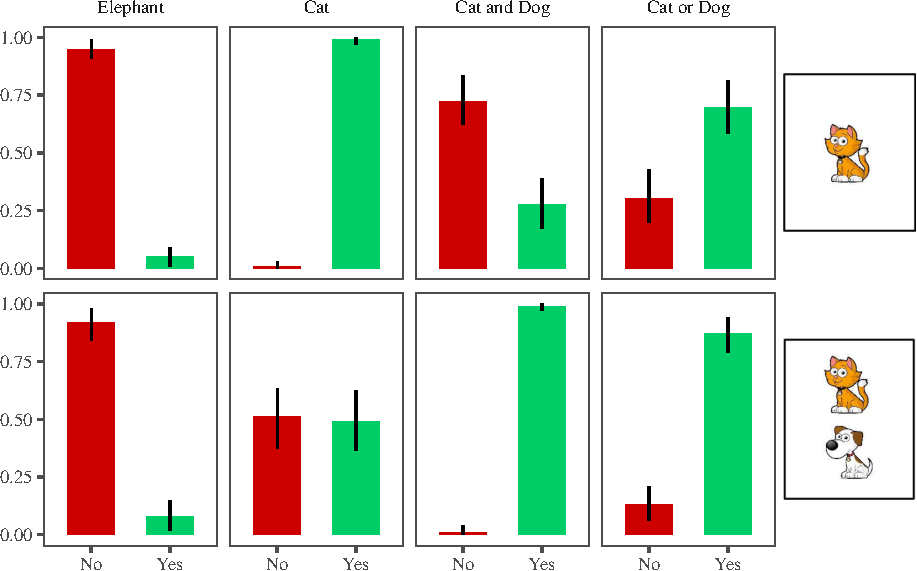
\includegraphics{Jasbi-Frank-2019_files/figure-latex/Study3tvjtPlot-1.pdf}
\caption{\label{fig:Study3tvjtPlot}Children's two-alternative foced-choice judgments in Experiment 3.}
\end{figure}

Figure \ref{fig:Study3tvjtPlot} shows children's 2AFC judgments. Starting with control trials, when the guessed animal (e.g. \emph{elephant}) was not on the card, children considered the guess \enquote{wrong}. When the guessed animal (e.g. \emph{cat}) was the only animal on the card (e.g. \textsc{cat}), children considered the guess \enquote{right}. However, if it was only one of the animals on the card (e.g. \textsc{cat+dog}), children were equally split between \enquote{wrong} and \enquote{right} judgments. This is in contrast to adults who unanimously considered such guesses as \enquote{right} in their 2AFC judgments (Figure \ref{fig:binaryAdultsPlot}). There are two possible explanations for this difference. First, some children may interpret a simple guess like \enquote{there is a cat} exhaustively as \enquote{there is \textbf{only} a cat}. Second, some children may consider leaving out an animal as a grave violation even though they do not interpret the guess as there is \textbf{only one} animal on the card. The first explanation is unexpected for a theory of acquisition that assumes children are overall more logical or literal as interpreters than adults (Noveck, 2001).

In conjunction trials, when the card had two animals (e.g. \textsc{cat+dog}) and both were guessed (e.g. \emph{cat and dog}) children unanimously considered the guess as \enquote{right}. When the card (e.g. \textsc{cat}) had only one of the gussed animals (e.g. \emph{cat and dog}), children were more likely to consider the guess \enquote{wrong}. This is similar to adults' binary judgments, but different in extent: adults were more consistent and unanimous in rejecting such guesses. In disjunction trials, when the card (e.g. \textsc{cat}) had only one of the guessed animals (e.g. \emph{cat or dog}), most children considered the guess \enquote{right}. This is again similar to adults but differs from them in extent: adults more consistently and unanimously judged such guesses as \enquote{right}. When the card had two animals (e.g. \textsc{cat+dog}) and both were guessed using a disjunction (e.g. \emph{cat or dog}), children considered the guess right.

\begin{figure}
\centering
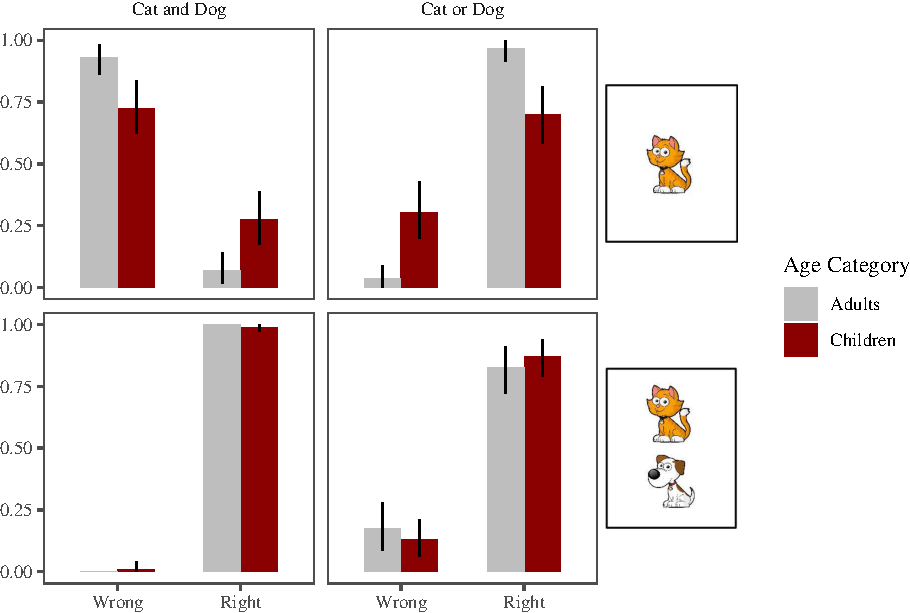
\includegraphics{Jasbi-Frank-2019_files/figure-latex/BinaryPlotComp-1.pdf}
\caption{\label{fig:BinaryPlotComp}The comparison of 2AFC judgment tasks for conjunction and disjunction trials in adults (Experiment 1) and children (Experiment 3).}
\end{figure}

Figure \ref{fig:BinaryPlotComp} provides a side-by-side comparison of adults' and children's 2AFC judgments for conjunction and disjunction trials. The judgments are very close and differ only very slighly in trial types where there is only one animal on the card. To quantify trial-type differences in adults and children, we fit separate Bayesian mixed-effects binomial logistic regressions for each group. To capture differences between adults and children, we fit a similar model to the combined dataset of adults and children and added age category (adult vs.~child) as an interaction term. As before, the model included the fixed dummy coded effect of trial-type (Levels: \enquote{one animal, \emph{or}} (reference) - \enquote{two animals, \emph{and}} - \enquote{one animal, \emph{and}} - \enquote{two animals, \emph{or}}). As before, the models had random intercepts and slopes for participants. Details of priors and convergence were similar to previous models as well.

\begin{figure}
\centering
\includegraphics{Jasbi-Frank-2019_files/figure-latex/exp3TVJTstats-1.pdf}
\caption{\label{fig:exp3TVJTstats}Left: Mean and 90\% highest posterior density interval for parameter values estimated in separate ordinal logistic regressions for adults and children, Right: Mean and 90\% highest posterior density interval for the interactive effect of age category (adult vs.~child) on 3AFC judgments.}
\end{figure}

The left panel of Figure \ref{fig:exp3TVJTstats} shows the mean and 90\% HPDI for three contrasts of interest estimated from separate binomial models for adults and children. The x-axis shows the contrasts between the following trial-types: conjunction vs.~disjunction trials when only one animal was on the card (one animal, \emph{and}-\emph{or}), trials with one vs.~two animals on the card when the guess was a disjunction (\emph{or}, two-one animal), and conjunction vs.~disjunction trials when two animals were on the card (two animals, \emph{and}-\emph{or}). Similar to the results reported in Experiment 2, adults' and children's estimated coefficients are similar in sign to one another, though adults' are more extreme in the first contrast. The first contrast (one animal, \emph{and}-\emph{or}) suggests that when only one animal was on the card, both adults and children had lower judgments for guesses with conjunction compared to guesses with disjunction. The second and third contrasts suggest that on average, children and adults did not differentiate between disjunction trial-types with one vs.~two animals or trial-types with two animals when the guess was a disjunction vs.~a conjunction. The majority considered all such trials as \enquote{right} in the binary truth value judgment task.

To understand the extent to which children's judgments differed from adults' we looked at the mean and the 90\% HPDIs of the interaction coefficients from the combined binomial model shown in the right panel of Figure \ref{fig:exp3TVJTstats}. We used this model to focus on the likely reliable differences between children and adults, even though they may be small. Based on the 90\% HPDIs, we can infer that judgments of adults and children differed in three ways. First, when the guess was a conjunction and only one animal was on the card, children were slightly more likely than adults to choose \enquote{right}. Second, when the guess was a disjunction and only one animal was on the card, children were slighly more likely to choose \enquote{wrong}. Notice that these two differences between children and adults are compatible with the label-matching account (Paris, 1973) but not the non-adult-like pragmatic enrichment account (Singh2016, Tieu et al., 2016). Under the pragmatic enrichment account, children should be more likely to say \enquote{wrong} to a disjunction with one disjunct true, but not more likely to say \enquote{right} to a conjunction when only one conjunct is true. Howver, the label-matching account predicts both these outcomes, because it posits that in both cases children disregard (or don't pay attention to) the connective and judge based on the match between labels and objects, which is partial in both cases.

Finally the third difference; our combined model suggested that children were slighly more likely than adults to judge the guess \enquote{right} when it was a disjunction and two animals were on the card. This is consistent with the hypothesis that children compute exclusivity implicatures at a lower rate than adults. However, as we will see in the next section, this hypothesis is undermined by the data from children's feedback, which point to children's sensitivity to the infelicity of disjunction when both disjuncts are true.

\textless{}--MIKE

\hypertarget{open-ended-feedback}{%
\subsubsection{Open-ended Feedback}\label{open-ended-feedback}}

\begin{figure}
\centering
\includegraphics{Jasbi-Frank-2019_files/figure-latex/exp3feedbackPlot-1.pdf}
\caption{\label{fig:exp3feedbackPlot}Children's Open-ended Feedback in Experiment 3.}
\end{figure}

Figure \ref{fig:exp3feedbackPlot} shows the distribution of children's feedback to the puppet in Experiment 3 (see Table \ref{tab:feedbackCat} for the definitions and examples of feedback categories). Similar to Experiment 2, Children's feedback showed four main patterns. First when the puppet guessed an animal not on the card (e.g. \emph{elephant}), there was a split pattern between negative judgments like \enquote{No!} and simply mentioning the animal on the card (e.g. \enquote{Cat!}). Second, almost all children responded with positive judgments like \enquote{Yes!} when the puppet's guess accurately matched what was on the card. This was the case in trials where there was only one animal on the card and the puppet mentioned it, as well as trials where there were two animals on the card and the puppet mentioned both with a conjunction. Third, children provided the largest number of corrective feedback in trials where the guess was either false or infelicitous. These included three trial types: (a) two animals on the card (e.g. \textsc{cat+dog}) but the puppet only guessed one (e.g. \emph{cat}); (b) the puppet guessed two animals with conjunction (e.g. \emph{cat and dog}) but only one of them was on the card (e.g. \textsc{cat}); and (c) two animals on the card (e.g. \textsc{cat+dog}), and the puppet guessed both but used a disjunction (e.g. \emph{cat or dog}). Finally, there was a pattern of feedback unique to disjunction trials with only one animal on the card. In such cases, almost all children simply named the animal on the card (e.g. \enquote{cat!}).

\begin{figure}
\centering
\includegraphics{Jasbi-Frank-2019_files/figure-latex/exp3FeedbackStats-1.pdf}
\caption{\label{fig:exp3FeedbackStats}The mean and 90\% highest posterior density interval of the coefficients of interest in experiment 3's mixed-effects multinomial logistic model on children's feedback.}
\end{figure}

MIKE----\textgreater{}To quantify and compare the distribution of children's feedback in connective trial-types, we used a Bayesian mixed-effects multinomial regression model with the fixed effect of trial-type as well as random intercepts and slopes for participants and items (cards). Similar to our analysis in Experiment 2, the dependent measure was children's feedback categories of judgment, description, and correction, with correction set as the reference category. The trial-types \enquote{one animal, \emph{or}}, \enquote{one animal, \emph{and}}, \enquote{two animals, \emph{and}} constituted the (dummy-coded) fixed effects of the model with \enquote{two animals, \emph{or}} set as the intercept. Priors and convergence information were identical to those reported for our previous models.

Figure \ref{fig:exp3FeedbackStats} shows the mean and 90\% HPDIs of the multinomial model co-efficients. These results replicate the findings on children's feedback reported in Experiment 2. Starting from the left, the HPDIs for judgments and descriptions over corrections for the \enquote{one animal, \emph{and}} trial-type included zero. This suggests that the feedback distribution was similar in conjunction trials with one animal and disjunction trials with two animals. Considering the \enquote{one animal, \emph{or}} trials, the HPDI for judgments over corrections included zero but not the HDPI for descriptions. This suggests that children provided more descriptions than corrections when only one of the disjuncts was true. Finally with \enquote{two animal, \emph{and}} trials, the HPDI for descriptions over corrections includes zero while that of judgments over corrections stays above zero. This suggests that when a conjunction was used and both animals were on the card, children provided more affirmative judgments than corrections. Overall, the results confirm the findings reported in Experiment 2: in connective trials, children were more likely to provide corrections in trial-types that were either false or infeliciotus. \textless{}----MIKE

\begin{figure}
\centering
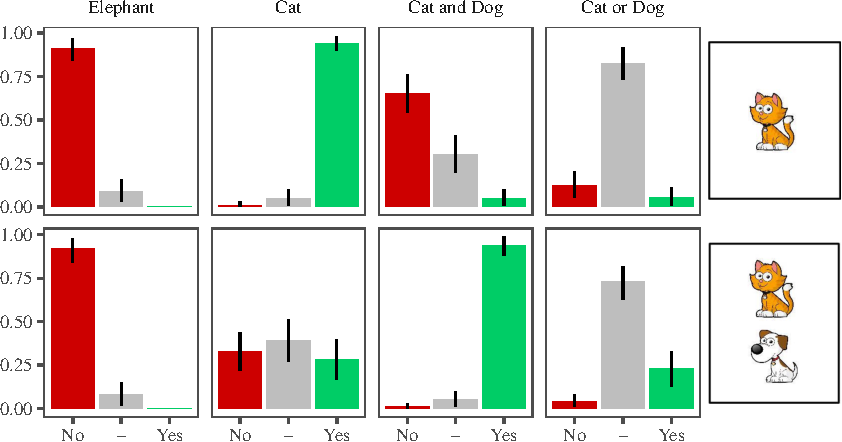
\includegraphics{Jasbi-Frank-2019_files/figure-latex/study3JudgmentPlot-1.pdf}
\caption{\label{fig:study3JudgmentPlot}Children's open-ended feedback in Experiment 3. The x-axis shows whether children spontaneously provided a yes (green), no (red), or other response (grey).}
\end{figure}

In Figure \ref{fig:study3JudgmentPlot} we break down children's open-ended feedback based on whether they spontaneously provided a simple judgment of \emph{Yes!} and \emph{No!}, or not. Responses that were not yes/no judgments are grouped in a middle category shown with a dash. The goal here is to compare children's open-ended and spontaneous binary judgments with their forced-choice binary judgments shown in Figure \ref{fig:Study3tvjtPlot}. Notice that both were provided in the same task and essentially one right after the other (forced-choice after spontaneous). Children's open-ended judgments and their forced choice judgments in study 3 show similar patterns for all types of guesses except for disjunctive ones. In trials that the puppet guessed a disjunction, the vast majority of children refused to provide a yes/no judgment when they were not forced to. Instead, they described the animal on the card or provided corrections to the puppet's infelicitous disjunctive guess.

One way to interpret these results is that disjunctive guesses (with at least one disjunct true) are considered neither right nor wrong. When children were forced to provide wrong/right responses in the experimental context, some conformed to the adult patterns of judgment and some did not. However, it is possible that such deviations from adult judgments do not reflect differences in the comprehension of disjunction, but rather differences in how children map their comprehension of disjunction onto the notions of \enquote{right} and \enquote{wrong} when forced to do so.

\begin{figure}
\centering
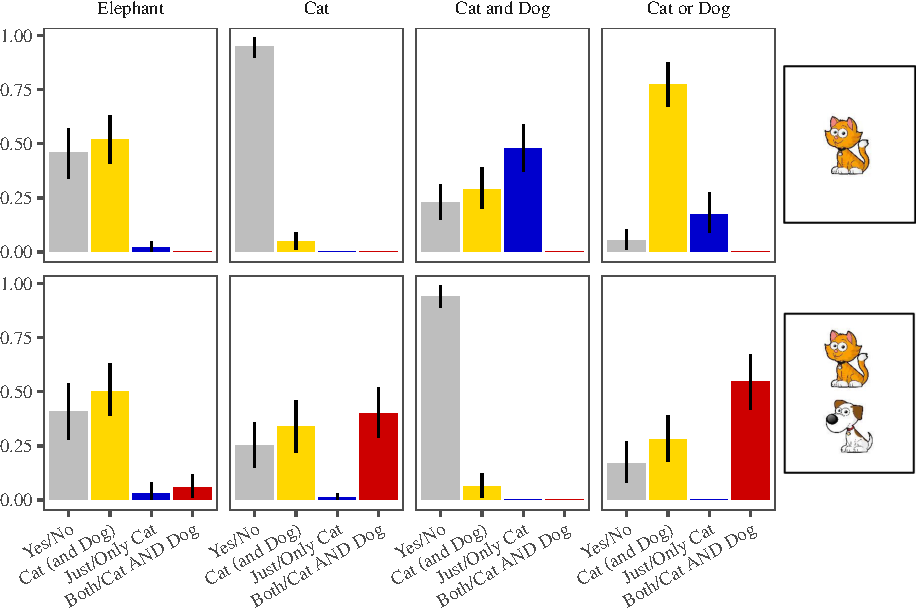
\includegraphics{Jasbi-Frank-2019_files/figure-latex/correctivePlot-1.pdf}
\caption{\label{fig:correctivePlot}Children's open-ended feedback in different trial types of Experiment 3.}
\end{figure}

Figure \ref{fig:correctivePlot} shows the proportion of feedback categories other than yes/no judgments on the x-axis. Our goal here is to display the trial types with corrective feedback (blue and red). These trial types include: (1) conjunction when only one conjunct is true (e.g.~guess: \emph{cat and a dog}, card: \textsc{cat}), (2) disjunction when both disjuncts are true (e.g.~guess: \emph{cat or dog}, card: \textsc{cat+dog}), and (3) simple guesses when two animals were on the card (e.g.~guess: \emph{cat}, \textsc{cat+dog}). As explained before, these trial types involved guesses that were either false or infelicitous. Furthermore, the type of corrective feedback children provided matched the type of mistakes made in the guesses. With conjunctive guesses (e.g. \emph{cat and a dog}) when there was only one animal on the card (e.g. \textsc{cat}), children provided exclusive corrections such as \enquote{just a cat} or \enquote{only a cat!}, suggesting that the other animal in the guess (e.g. \emph{dog}) should have been excluded. When two animals were on the card (e.g. \textsc{cat+dog}) and the puppet used a disjunctive guess (e.g. \emph{cat or dog}), or a simple guess (e.g. \emph{cat}), children provided inclusive feedback such as \enquote{cat AND dog} or \enquote{both}, suggesting that another animal should have been included. This is particularly notable in the case of disjunction since both animals were mentioned, but children still emphasized that the connective \emph{and} should have been used, or that \emph{both} animals mentioned were actually on the card. Such corrective comments hint at a deeper understanding of differences between the meaning of disjunction and conjunction.

\hypertarget{discussion-2}{%
\subsection{Discussion}\label{discussion-2}}

Experiment 3 measured children's comprehension of logical connectives in two ways: First, with analyzing their open-ended feedback and second, with a two-alternative forced choice task. First, we asked children to say \emph{yes} to the puppet if he was right and \emph{no} if he was wrong. However, children could provide any form of feedback they wanted. Second, we followed children's open-ended feedback with a 2AFC question: \enquote{Was the puppet right?} This way, we could measure children's comprehension in two different ways in the same trial. Ideally, both measures should show similar results. However, the findings were similar for conjunctive guesses, but not disjunctive ones. Children avoided binary right/wrong feedback with disjunction and preferred to provide more nuanced feedback.

The 2AFC responses followed the predicted pattern: conjunctive guesses were judged wrong if only one conjunct was true, and right if both were true. Disjunctive guesses were judged right whether one or both disjuncts were true. There was no significant difference in the 2AFC task between the responses of children and those of adults in Experiment 1. Children's open-ended feedback in Experiment 3 replicated the findings of Experiment 2. Children provided more corrective feedback in false and infelicitous trials than in true and felicitous ones. The corrective feedback was tailored to the puppet's mistake. If the puppet used a conjunction when there was only one animal on the card, children pointed out that the other animal should have been excluded from the guess. They used the exclusive adverbials \emph{just} and \emph{only} in their feedback. If the puppet used a disjunction when both animals were on the card, children stressed \emph{and} or \emph{both}, implying that both animals should have been included.

While the 2AFC results suggested that children took no issue with disjunctive guesses when both disjuncts were true, the analysis of their corrective feedback showed that they provide appropriate corrections in such cases and emphasized that the connective \emph{and} would have been a better guess. Taking both measures together, we conclude that even though children are aware of the problem with such guesses, they do not consider them \emph{wrong}.

\hypertarget{general-discussion}{%
\section{General Discussion}\label{general-discussion}}

We reported three studies on adults' and preschool children's comprehension of disjunction. The first study used two- and three-alternative forced choice judgment tasks with adults. In the 2AFC task, adult interpretations closely matched the semantic accounts of \emph{and} and \emph{or} as conjunction and inclusive disjunction. The 2AFC judgments did not register robust signs of pragmatic infelicities. However, the 3AFC judgments showed signs of pragmatic infelicities, especially in disjunctive guesses with true disjuncts. When two animals where on the card (e.g.~cat and dog) and the guess used \emph{or} (e.g. \emph{There is a cat or a dog!}), participants were more likely to choose \enquote{kinda right} rather than \enquote{right}.

The second study used a 3AFC judgment task with four-year-old children. It also included an exploratory analysis of children's open-ended verbal feedback to the puppet in the experimental setting. Children's interpretations were similar to those of adults in the 3AFC task and only differed for pragmatically infelicitous disjunctions. When both disjuncts were true, adults tended to judge disjunctive guesses as \enquote{kinda right}. This was evidence for the pragmatic infelicity of such guesses. While, children judged such disjunctive statement as \enquote{right}, the analysis of their open-ended feedback showed that they took issue with such statements as well, and provided appropriate corrective feedback.

In the third study, we focused on eliciting open-ended verbal feedback from children and followed it with a 2AFC question. Children's 2AFC responses reflected the semantics of the connectives \emph{and} and \emph{or} as conjunction and inclusive disjunction. There was no significant difference between children and adults in the 2AFC task. Analysis of children's open-ended feedback replicated the findings in study 2. Children provided more corrective feedback in false and pragmatically infelicitous trials with the connectives than in felicitous trials. The comparison of the 2AFC task and children's open-ended responses showed that children are sensitive to the infelicity of disjunctions with true disjuncts, even though they consider them to be \enquote{right} guesses.

Previous studies had suggested that adults and preschool children differ in their interpretation of disjunction in two ways. First, unlike adults, children might interpret a disjunction as conjunction (Singh et al., 2016; Tieu et al., 2016). Second, children might interpret \emph{or} as inclusive disjunction when adults interpret it as exclusive (Crain, 2012). The studies reported here provide evidence for the hypothesis that these differences may be an artifact of the experimental task and the type of measurement (Skordos et al. (n.d.), Katsos (2014)).

Considering the first difference, in the 2AFC and 3AFC judgment tasks we found only small (but significant) preferences for both disjuncts being true rather than only one. Combining the 2AFC and the verbal feedback results, we expect that a child with strong conjunctive interpretation of disjunction should have rejected a disjunctive guess when only one disjunct was true, provided a \enquote{Just/Only} feedback, and accepted the guess when both disjuncts were true without providing a correction. We found no child in our sample that showed this pattern of responses. Two children who consistently rejected a disjunction when only one disjunct was true, provided corrective feedback when one or both disjuncts were true. Therefore while it is possible that some children interpret \emph{or} as \emph{and}, our results did not show a common or consistent effect.

We would like to add that conjunctive interpretations of disjunction, even when robustly observed, can have at least two potential explanations. First, non-linguistic interpretive strategies and preferences, due to task demands or unknown connective meaning (Clark, 1973; Paris, 1973), and second, non-adult-like pragmatic enrichment, hypothesized to occur in free-choice contexts in adult language (Singh et al., 2016; Tieu et al., 2016). As explained in section \ref{litreview}, previous research provides substantial evidence for task-related increase in conjunctive readings of disjunction (Braine \& Rumain, 1981; Neimark \& Slotnick, 1970; Paris, 1973; Skordos et al., n.d.). In order to show instances of pragmatically enriched conjunctive readings in preschool children, it is important to first rule out task-related conjunctive interpretations.

Considering the second difference, namely the lower rate of exclusivity inferences in preschool children, our studies provided evidence that the choice of measurement may play an important role. In the 3AFC judgment task when two animals were on the card (e.g.~card: cat and dog, guess: \enquote{There is a cat or a dog}), adults were more likely to choose \enquote{kinda right} than children were. Children mostly chose \enquote{right}. However, in their free-form feedback, children corrected such utterances and suggested that the connective \emph{and} should have been used instead of \emph{or}.

There have been at least four major proposals to account for children's perceived low rate of \enquote{implicature computation}: processing difficulty (Pouscoulous, Noveck, Politzer, \& Bastide, 2007; Reinhart, 2004), non-adult-like lexical entry (Barner et al., 2011; Horowitz, Schneider, \& Frank, 2017), pragmatic tolerance (Katsos \& Bishop, 2011), and the role of experimental measurement (Katsos, 2014). Below we argue that the first three cannot explain the reported results of children's forced judgments and free-form feedback, and that these results highlight the role of experimental measurement as a source of perceived differences in children and adults pragmatic inferences.

\textbf{1. Processing difficulty.} First, processing accounts locate the problem in children's processing capacities such as working memory. They suggest that pragmatic computations are cognitively taxing and children lack the appropriate processing resources to carry them out appropriately. A prediction of processing accounts (at least in their current format) is that children will show reduced implicature computations for all types of implicatures -- scalar or not. This prediction was not borne out in our experimental results here. In Experiment 3, children were much more likely than adults to call a simple guess (e.g. \emph{There is a cat!}) \enquote{wrong} if there were two animals on the card (e.g.~cat and dog). In other words, children's interpretations were much more exhaustive than adults. Processing accounts do not predict that children may derive implicatures at a higher rate than adults but this is what we found, at least for the traditional interpretation of the judgment task.

\textbf{2. Non-adult-like Lexicon.} Several proposals blame the structure of the child's lexicon for the alleged failure in deriving implicatures. The assumption is that the child's lexical entry for scalar items must include three elements for successful derivation: 1. the semantics of the weak term (e.g. \emph{some}, \emph{or}) 2. the semantics of the strong term (e.g. \emph{all},\emph{and}); and possibly 3. a scale that recognizes the stronger term as an alternative to the weaker one (e.g. \textless{}\emph{some}, \emph{all}\textgreater{}, \textless{}\emph{or}, \emph{and}\textgreater{}). Each of these elements have been pinpointed as the source of the problem in previous studies (Barner et al., 2011; Horowitz et al., 2017; Katsos \& Bishop, 2011). However none of them seem to apply to the results reported here.

If children in this study lack the semantics of the connective \emph{or}, we would expect them to either perform at chance or default to a conjunctive interpretation. Neither prediction was borne out in studies 2 and 3. Furthermore, children's free-form linguistic feedback in both studies suggested that children understood disjunction well enough to provide relevant feedback. So this explanation seems unlikely. The problem cannot be that children do not know the meaning of \emph{and} either. Children's performance in both study 2 and 3 for conjunction trials show that they understand its meaning very well. Finally, comparing children's truth value judgments and their free-form verbal feedback, we found that many children judged a disjunction with true disjuncts as \enquote{right}, yet went on to correct the puppet and explicitly mention \emph{and} as the connective he should have used. If children could not access the stronger alternative, they could not have mentioned it in their feedback either. And if accessing the stronger alternative would have resulted in expressing sub-optimal judgments, they should not have judged the guess as \enquote{right}.

\textbf{3. Pragmatic Tolerance.} Katsos \& Bishop (2011) suggested that children tend to tolerate pragmatic infelicities more than adults. They showed that when children were provided with a 2AFC judgment task, they considered a description with the scalar term \emph{some} as \enquote{right} when \emph{all} was more informative (e.g. \emph{The turtle played with some of the balls.}, Scene: the turtle played with all the balls.) However, when they are presented with three options (small, big, and huge strawberries) in a 3AFC task, they choose the middle option in the same type of trials. They argued that children tolerate pragmatic infelicities and do not regard them as \enquote{wrong}. As in a processing account, the tolerance account predicts that scalar and ad-hoc implicatures will be similarly affected. However, our results did not match those of Katsos \& Bishop (2011). When children were presented with a 3AFC task, they chose the highest reward (and not the middle option) for uses of \emph{or} when \emph{and} was more informative. Second, and more importantly, we found different patterns for exhaustive and scalar inferences as mentioned before. This is not predicted by the tolerance account unless we assume that children are more tolerant towards violations of scalar inferences than they are towards exhaustive ones. While this is not currently assumed in the literature, it is a possible adjustment. However, we would like address this issue by focusing on another related factor: the role of measurement in estimates of children's pragmatic capacity (Katsos, 2014).

\textbf{4. The Role of Measurment.} Two observations in the current studies provide support for the hypothesis that methodological issues, and more specifically issues of measurement contribute to the differences found between adults and children in pragmatic capacity. First, Experiment 1 showed that even for adults, the estimates of adult infelicity rates may differ based on the number of alternatives in the forced choice task. A 2AFC task underestimated adults' sensitivity to pragmatic infelicity. In fact, in a follow up study, we systematically varied the number of response options and replicated the results presented here (see Jasbi et al., 2019). Second, children's open-ended linguistic feedback in the experimental context better reflected their sensitivity to pragmatic nuances than the forced-choice judgment tasks. Third, children showed a higher rate of \enquote{wrong} judgments for cases of exhaustive inferences (simple guesses with two animals on the card) than adults did. While a difference in sensitivity to ad-hoc vs.~scalar implicatures has been reported and argued for before (Horowitz et al., 2017; Stiller, Goodman, \& Frank, 2015), a higher sensitivity than adults is not predicted by any of the current accounts.

\begin{figure}
\centering
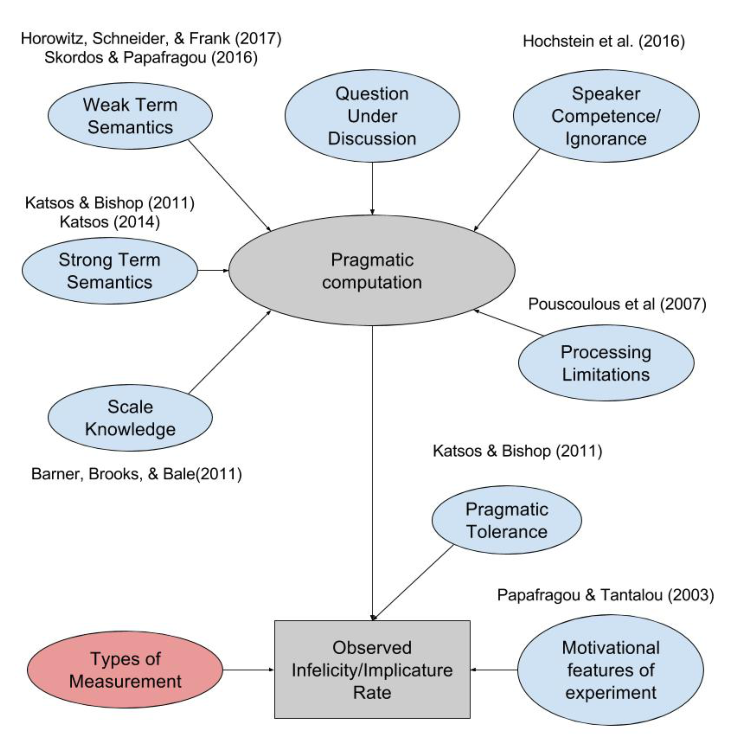
\includegraphics{Jasbi-Frank-2019_files/figure-latex/implicatureGraph-1.pdf}
\caption{\label{fig:implicatureGraph}Factors that could affect pragmatic computations and the estimates of these computations in the experimental settings}
\end{figure}

Figure \ref{fig:implicatureGraph} shows a summary of the factors that are proposed to affect pragmatic computations. As Pouscoulous \& Noveck (2009) and Katsos (2014) have suggested, the central issue is \enquote{the rate} at which children and adults manifest pragmatic reasoning in the experimental setting. No one doubts children's capacity to perform such computations. At issue is the extent to which children and adults compute specific implicatures. As Katsos (2014) pointed out, it seems reasonable to assume that all these factors play some part here. What matters is the degree to which each contributes to the outcome.

The results of the studies reported here suggest that it is important to distinguish between factors that affect pragmatic computations and those that affect the observed \enquote{rate} in an experimental setting. As we showed in Experiment 1, given the number of alternatives in the forced choice task (2AFC vs.~3AFC), we may get different estimates of adults' rate of infelicity judgments, but we cannot assume that there is a difference in adults' pragmatic capacities in these two tasks. A similar situation exists when we compare children's forced choice measures of infelicity and their open-ended feedback.

In order to better understand the differences between adults and children's semantic and pragmatic capacities, it is necessary to have a good understanding of how our measurements affect estimates of adults and children's performance in the experimental tasks. Children may be no more capable of making exhaustive inferences than adults and no less capable of making scalar inferences either. They may simply have a different construal of the wrong-right scale and of what the forced-choice task is about. The concepts \enquote{right} and \enquote{wrong} are as much subject to developmental change and differences between adults and children as are scalar items that constitute the focus of our studies. Relying on a single type of measurement increases the risk of measurement-specific conclusions. Using multiple measurements in the same task can provide converging evidence for felicity/infelicity or presence/absence of specific inferences. Ultimately, in order to capture semantic and pragmatic competences of adults and (especially) children, we need to develop methods that can reliably tap into specific dimensions of meaning.

\hypertarget{conclusion}{%
\subsection{Conclusion}\label{conclusion}}

We provided three studies that tested adults and children's comprehension of disjunction in existential sentences using three different measures: binary forced-choice truth value judgments (2AFC task), ternary forced-choice truth value judgments (3AFC task), and free-form verbal feedback. The results suggested that for each population, different measures were sensitive to different aspects of meaning. The binary measure captured children and adults intutions about truth values well: it showed that they considered a disjunction as inclusive in existential sentences of the guessing game. Ternary judgments provided evidence for adults' pragmatic inferences: adults often considered a disjunction when both disjuncts were true as \enquote{kinda right} and not completely right. For children, the ternary judgments did not register such an effect, but their free-form verbal feedback did. When both disjuncts were true, children verbally corrected the puppet and suggested that he should have said \emph{and} instead of \emph{or}. The combination of children's truth valued judgments and their verbal feedback suggested that on average, children in our sample understood that when both propositions were true, the conjunction and disjunction of them were also true, yet conjunction made a more appropriate and felicitous utterance.

Since Tarski's original observations on disjunction, research in semantics and pragmatics has shown that the variety of interpretations Tarski observed are in fact distinct types of meaning observed in many aspected of langauge and connected to distinct processes that generate them. Therefore, while the inclusive interpretation is hypothesized to be part of \emph{or}'s semantics, exclusivity and ignorance interpretations are analyzed as distinct pragmatic inferences generated separately. This theoretical insight has in turn lead developmental researchers to seek distinct developmental mechanisms for each type of meaning. The results of the studies reported here suggest that as more and more varieties of meaning become subject of experimental studies, we also need to develop measures especially suited to capture the specific aspect of meaning under investigation.

\newpage

\hypertarget{references}{%
\section{References}\label{references}}

\newpage

\hypertarget{supplementary-materials}{%
\section{Supplementary Materials}\label{supplementary-materials}}

\begin{figure}

{\centering 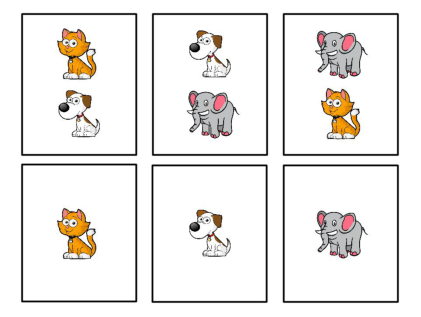
\includegraphics{Jasbi-Frank-2019_files/figure-latex/stimuli-1} 

}

\caption{Cards used in the connective guessing game.}\label{fig:stimuli}
\end{figure}

\begin{figure}
\centering
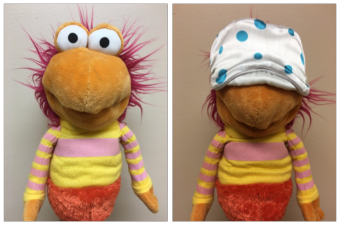
\includegraphics{Jasbi-Frank-2019_files/figure-latex/jazzy-1.pdf}
\caption{\label{fig:jazzy}The puppet, Jazzy, with and without the sleeping mask.}
\end{figure}

\begin{longtable}[]{@{}lll@{}}
\caption{\label{tab:instruction} Instruction Trials.}\tabularnewline
\toprule
Card & Guess & Reward\tabularnewline
\midrule
\endfirsthead
\toprule
Card & Guess & Reward\tabularnewline
\midrule
\endhead
CAT & There is a dog! & Circle\tabularnewline
ELEPHANT & There is an elephant! & Big Star\tabularnewline
CAT-DOG & There is a dog! & Little Star\tabularnewline
\bottomrule
\end{longtable}

\begin{longtable}[]{@{}lll@{}}
\caption{\label{tab:instructionStudy3} Instruction Trials for Experiment 3.}\tabularnewline
\toprule
Card & Guess & Response\tabularnewline
\midrule
\endfirsthead
\toprule
Card & Guess & Response\tabularnewline
\midrule
\endhead
CAT & there is a dog! & No!\tabularnewline
ELEPHANT & there is an elephant! & Yes!\tabularnewline
DOG-ELEPHANT & there is a cat! & No!\tabularnewline
DOG & there is a dog! & Yes!\tabularnewline
\bottomrule
\end{longtable}

\begin{longtable}[]{@{}lll@{}}
\caption{\label{tab:feedbackCat} Definitions and Examples for the Feedback Categories.}\tabularnewline
\toprule
\begin{minipage}[b]{0.14\columnwidth}\raggedright
Category\strut
\end{minipage} & \begin{minipage}[b]{0.46\columnwidth}\raggedright
Definition\strut
\end{minipage} & \begin{minipage}[b]{0.31\columnwidth}\raggedright
Examples\strut
\end{minipage}\tabularnewline
\midrule
\endfirsthead
\toprule
\begin{minipage}[b]{0.14\columnwidth}\raggedright
Category\strut
\end{minipage} & \begin{minipage}[b]{0.46\columnwidth}\raggedright
Definition\strut
\end{minipage} & \begin{minipage}[b]{0.31\columnwidth}\raggedright
Examples\strut
\end{minipage}\tabularnewline
\midrule
\endhead
\begin{minipage}[t]{0.14\columnwidth}\raggedright
\textbf{None}\strut
\end{minipage} & \begin{minipage}[t]{0.46\columnwidth}\raggedright
no verbal feedback\strut
\end{minipage} & \begin{minipage}[t]{0.31\columnwidth}\raggedright
\strut
\end{minipage}\tabularnewline
\begin{minipage}[t]{0.14\columnwidth}\raggedright
\textbf{Judgment}\strut
\end{minipage} & \begin{minipage}[t]{0.46\columnwidth}\raggedright
provided verbal judgment mirroring the reward\strut
\end{minipage} & \begin{minipage}[t]{0.31\columnwidth}\raggedright
\enquote{No!}, \enquote{Yes!} , \enquote{You are right!}\strut
\end{minipage}\tabularnewline
\begin{minipage}[t]{0.14\columnwidth}\raggedright
\textbf{Description}\strut
\end{minipage} & \begin{minipage}[t]{0.46\columnwidth}\raggedright
mentioned the animal(s) on the card\strut
\end{minipage} & \begin{minipage}[t]{0.31\columnwidth}\raggedright
\enquote{elephant}, \enquote{cat and dog}\strut
\end{minipage}\tabularnewline
\begin{minipage}[t]{0.14\columnwidth}\raggedright
\textbf{Correction}\strut
\end{minipage} & \begin{minipage}[t]{0.46\columnwidth}\raggedright
used focus particles like \emph{only}/\emph{just}, emphasized \emph{and} or used \emph{both}\strut
\end{minipage} & \begin{minipage}[t]{0.31\columnwidth}\raggedright
\enquote{only cat}, \enquote{just elephant}, \enquote{both!}, \enquote{cat AND dog!}\strut
\end{minipage}\tabularnewline
\bottomrule
\end{longtable}

\setlength{\parindent}{-0.5in}
\setlength{\leftskip}{0.5in}

\hypertarget{refs}{}
\leavevmode\hypertarget{ref-barner2011accessing}{}%
Barner, D., Brooks, N., \& Bale, A. (2011). Accessing the unsaid: The role of scalar alternatives in children's pragmatic inference. \emph{Cognition}, \emph{118}(1), 84--93.

\leavevmode\hypertarget{ref-barr2013random}{}%
Barr, D. J., Levy, R., Scheepers, C., \& Tily, H. J. (2013). Random effects structure for confirmatory hypothesis testing: Keep it maximal. \emph{Journal of Memory and Language}, \emph{68}(3), 255--278.

\leavevmode\hypertarget{ref-braine1981development}{}%
Braine, M. D., \& Rumain, B. (1981). Development of comprehension of ``or'': Evidence for a sequence of competencies. \emph{Journal of Experimental Child Psychology}, \emph{31}(1), 46--70.

\leavevmode\hypertarget{ref-burkner2017brms}{}%
Bürkner, P.-C. (2017). Brms: An r package for bayesian multilevel models using stan. \emph{Journal of Statistical Software}, \emph{80}(1), 1--28.

\leavevmode\hypertarget{ref-chierchia2001acquisition}{}%
Chierchia, G., Crain, S., Guasti, M. T., Gualmini, A., \& Meroni, L. (2001). The acquisition of disjunction: Evidence for a grammatical view of scalar implicatures. In \emph{Proceedings of the 25th Boston University conference on language development} (pp. 157--168). Somerville, MA: Cascadilla Press.

\leavevmode\hypertarget{ref-chierchia1998some}{}%
Chierchia, G., Crain, S., Guasti, M. T., \& Thornton, R. (1998). ``Some'' and ``or'': A study on the emergence of logical form. In \emph{Proceedings of the Boston University conference on language development} (Vol. 22, pp. 97--108). Somerville, MA: Cascadilla Press.

\leavevmode\hypertarget{ref-chierchia2004semantic}{}%
Chierchia, G., Guasti, M. T., Gualmini, A., Meroni, L., Crain, S., \& Foppolo, F. (2004). Semantic and pragmatic competence in children's and adults' comprehension of or. In I. Noveck \& D. Sperber (Eds.), \emph{Experimental pragmatics} (pp. 283--300). Basingstoke: Palgrave Macmillan.

\leavevmode\hypertarget{ref-clark1973non}{}%
Clark, E. V. (1973). Non-linguistic strategies and the acquisition of word meanings. \emph{Cognition}, \emph{2}(2), 161--182.

\leavevmode\hypertarget{ref-crain2008interpretation}{}%
Crain, S. (2008). The interpretation of disjunction in universal grammar. \emph{Language and Speech}, \emph{51}(1-2), 151--169.

\leavevmode\hypertarget{ref-crain2012emergence}{}%
Crain, S. (2012). \emph{The emergence of meaning}. Cambridge: Cambridge University Press.

\leavevmode\hypertarget{ref-crain2000acquisition}{}%
Crain, S., Gualmini, A., \& Meroni, L. (2000). The acquisition of logical words. \emph{LOGOS and Language}, \emph{1}, 49--59.

\leavevmode\hypertarget{ref-goro2004acquisition}{}%
Goro, T., \& Akiba, S. (2004). The acquisition of disjunction and positive polarity in Japanese. In \emph{Proceedings of the 23rd West Coast conference on formal linguistics} (pp. 251--264). Somerville, MA: Cascadilla Press.

\leavevmode\hypertarget{ref-grice1975logic}{}%
Grice, H. P. (1975). Logic and conversation. \emph{1975}, 41--58.

\leavevmode\hypertarget{ref-gualminicrain2002}{}%
Gualmini, A., \& Crain, S. (2002). Why no child or adult must learn de Morgan's laws. In \emph{Proceedings of the Boston University conference on language development}. Somerville, MA: Cascadilla Press.

\leavevmode\hypertarget{ref-gualmini2000}{}%
Gualmini, A., Crain, S., \& Meroni, L. (2000). Acqisition of disjunction in conditional sentences. In \emph{Proceedings of the boston university conference on language development}.

\leavevmode\hypertarget{ref-horowitz2017trouble}{}%
Horowitz, A. C., Schneider, R. M., \& Frank, M. C. (2017). The trouble with quantifiers: Exploring children's deficits in scalar implicature. \emph{Child Development}.

\leavevmode\hypertarget{ref-piaget1958growth}{}%
Inhelder, B., \& Piaget, J. (1958). \emph{The growth of logical thinking from childhood to adolescence: An essay on the construction of formal operational structures} (Vol. 84). London: Routledge.

\leavevmode\hypertarget{ref-jasbi2019linking}{}%
Jasbi, M., Waldon, B., \& Degen, J. (2019). Linking hypothesis and number of response options modulate inferred scalar implicature rate. \emph{Frontiers in Psychology}, \emph{10}.

\leavevmode\hypertarget{ref-johansson1975preschool}{}%
Johansson, B. S., \& Sjolin, B. (1975). Preschool children's understanding of the coordinators ``and'' and ``or''. \emph{Journal of Experimental Child Psychology}, \emph{19}(2), 233--240.

\leavevmode\hypertarget{ref-katsos2014scalar}{}%
Katsos, N. (2014). Scalar implicature. In D. Matthews (Ed.), \emph{Pragmatic development in first language acquisition} (Vol. 10, p. 183---198). Amsterdam: John Benjamins.

\leavevmode\hypertarget{ref-katsos2011pragmatic}{}%
Katsos, N., \& Bishop, D. V. (2011). Pragmatic tolerance: Implications for the acquisition of informativeness and implicature. \emph{Cognition}, \emph{120}(1), 67--81.

\leavevmode\hypertarget{ref-neimark1970}{}%
Neimark, E. D. (1970). Development of comprehension of logical connectives: Understanding of ``or''. \emph{Psychonomic Science}, \emph{21}(4), 217--219.

\leavevmode\hypertarget{ref-neimarkSlotnick1970}{}%
Neimark, E. D., \& Slotnick, N. S. (1970). Development of the understanding of logical connectives. \emph{Journal of Educational Psychology}, \emph{61}(6p1), 451.

\leavevmode\hypertarget{ref-nitta1966basic}{}%
Nitta, N., \& Nagano, S. (1966). Basic logical operations and their verbal expressions: Child's conception of logical sum and product. \emph{Research Bulletin of the National Institute for Educational Research, Tokyo}, \emph{7}, 1--27.

\leavevmode\hypertarget{ref-notley2012notevery}{}%
Notley, A., Thornton, R., \& Crain, S. (2012a). English-speaking children's interpretation of disjunction in the scope of ``not every''. \emph{Biolinguistics}, \emph{6}(1), 32--69.

\leavevmode\hypertarget{ref-notley2012children}{}%
Notley, A., Zhou, P., Jensen, B., \& Crain, S. (2012b). Children's interpretation of disjunction in the scope of ``before'': A comparison of English and Mandarin. \emph{Journal of Child Language}, \emph{39}(03), 482--522.

\leavevmode\hypertarget{ref-noveck2001children}{}%
Noveck, I. A. (2001). When children are more logical than adults: Experimental investigations of scalar implicature. \emph{Cognition}, \emph{78}(2), 165--188.

\leavevmode\hypertarget{ref-papafragou2003scalar}{}%
Papafragou, A., \& Musolino, J. (2003). Scalar implicatures: Experiments at the semantics--pragmatics interface. \emph{Cognition}, \emph{86}(3), 253--282.

\leavevmode\hypertarget{ref-paris1973comprehension}{}%
Paris, S. G. (1973). Comprehension of language connectives and propositional logical relationships. \emph{Journal of Experimental Child Psychology}, \emph{16}(2), 278--291.

\leavevmode\hypertarget{ref-pouscoulous2009going}{}%
Pouscoulous, N., \& Noveck, I. A. (2009). Going beyond semantics: The development of pragmatic enrichment. In S. Foster-Cohen (Ed.), \emph{Language acquisition} (pp. 196--215). Berlin: Springer.

\leavevmode\hypertarget{ref-pouscoulous2007developmental}{}%
Pouscoulous, N., Noveck, I. A., Politzer, G., \& Bastide, A. (2007). A developmental investigation of processing costs in implicature production. \emph{Language Acquisition}, \emph{14}(4), 347--375.

\leavevmode\hypertarget{ref-reinhart2004processing}{}%
Reinhart, T. (2004). The processing cost of reference set computation: Acquisition of stress shift and focus. \emph{Language Acquisition}, \emph{12}(2), 109--155.

\leavevmode\hypertarget{ref-Singh2016}{}%
Singh, R., Wexler, K., Astle-Rahim, A., Kamawar, D., \& Fox, D. (2016). Children interpret disjunction as conjunction: Consequences for theories of implicature and child development. \emph{Natural Language Semantics}, \emph{24}(4), 305--352.

\leavevmode\hypertarget{ref-skordosEtal2018}{}%
Skordos, D., Feiman, R., Bale, A., \& Barner, D. (n.d.). \emph{Do children interpret ``or'' conjunctively?} Retrieved from \url{https://osf.io/2srxk/}

\leavevmode\hypertarget{ref-stiller2015ad}{}%
Stiller, A. J., Goodman, N. D., \& Frank, M. C. (2015). Ad-hoc implicature in preschool children. \emph{Language Learning and Development}, \emph{11}(2), 176--190.

\leavevmode\hypertarget{ref-su2014acquisition}{}%
Su, Y. (2014). The acquisition of logical connectives in child Mandarin. \emph{Language Acquisition}, \emph{21}(2), 119--155.

\leavevmode\hypertarget{ref-su2013disjunction}{}%
Su, Y., \& Crain, S. (2013). Disjunction and universal quantification in child mandarin. \emph{Language and Linguistics}, \emph{14}(3), 599--631.

\leavevmode\hypertarget{ref-suppes1969young}{}%
Suppes, P., \& Feldman, S. (1969). \emph{Young children's comprehension of logical connectives.} \emph{ERIC}. Department of Health, Education, Welfare. Office of Education.

\leavevmode\hypertarget{ref-tarski1941logic}{}%
Tarski, A. (1941). \emph{Introduction to logic and to the methodology of the deductive sciences}. Oxford University Press.

\leavevmode\hypertarget{ref-tieu2016}{}%
Tieu, L., Yatsushiro, K., Cremers, A., Romoli, J., Sauerland, U., \& Chemla, E. (2016). On the role of alternatives in the acquisition of simple and complex disjunctions in french and japanese. \emph{Journal of Semantics}.


\end{document}
